\documentclass[10pt,a4paper]{book}

\usepackage{amsmath}

\usepackage{inputenc}
\usepackage{fvextra}

\usepackage{algpseudocode}
\usepackage{algorithmicx}
\usepackage{amsfonts}
\usepackage{amssymb}
\usepackage{amsthm}
\usepackage[spanish]{babel}
\usepackage{bm}
\usepackage{booktabs} % To thicken table lines
\usepackage{bussproofs}
\usepackage{caption}
\usepackage{csquotes}
\usepackage{colortbl}
\usepackage{dsfont}
\usepackage{environ}
\usepackage[shortlabels]{enumitem}
\usepackage{fancyhdr}
\usepackage{forest}
\usepackage{geometry}
\usepackage{graphicx}
\usepackage[hidelinks]{hyperref}
\usepackage{ifthen}
\usepackage{multicol}
\usepackage{multirow}
\usepackage{sidecap}
\usepackage{stmaryrd}
\usepackage{tabularx}
\usepackage{titling}
\usepackage{tikz}
\usepackage{xcolor}
\usepackage{wrapfig}
\usepackage{minted}

\usetikzlibrary{arrows}
\usetikzlibrary{arrows.meta}
\usetikzlibrary{automata}
\usetikzlibrary{calc}
\usetikzlibrary{fit}
\usetikzlibrary{matrix}
\usetikzlibrary{positioning}
\usetikzlibrary{shapes.geometric}
\usetikzlibrary{shapes.multipart}


\title{Teoría de Lenguajes}
\author{Gianfranco Zambonni}
%%%% CONFIGURACIONES %%%%

%% La coma de los reales es un punto
\decimalpoint{}

%%% Tamaño de pagina
%\geometry{
%	includeheadfoot,
%	left=2.54cm,
%	bottom=1cm,
%	top=1cm,
%	right=2.54cm
%}

%\stul{0.1cm}{0.2ex}

%% HEADER Y FOOTER
\pagestyle{fancy}

\fancyhf{}

\fancyhead[LO]{\rightmark} % \thesection\ 
\fancyhead[RO]{\small{\thetitle}}
\fancyfoot[CO]{\thepage}
\renewcommand{\headrulewidth}{0.5pt}
\renewcommand{\footrulewidth}{0.5pt}
\setlength{\headsep}{1cm}
\setlength{\headheight}{13.07225pt}

\renewcommand{\baselinestretch}{1.2}  % line spacing

%% Links en indice 
\hypersetup{
	linktoc=all,     %set to all if you want both sections and subsections linked
	linkcolor=blue,  %choose some color if you want links to stand out
}
\definecolor{darkgreen}{rgb}{0.0, 0.5, 0.0}

\newcommand{\red}[1]{{\color{red}#1}}
\newcommand{\blue}[1]{{\color{blue}#1}}
\newcommand{\green}[1]{{\color{darkgreen}#1}}

\newcommand{\deriva}{\overset{*}{\Rightarrow}}
\newcommand{\iffa}[1]{
  \underset{\text{#1}}{\iff}
}
\newcommand{\iffab}[2]{
  \underset{\text{#2}}{\iffa{#1}}
}

\newcommand{\thena}[1]{
  \underset{\text{#1}}{\implies}
}
\newcommand{\thenab}[2]{
  \underset{\text{#2}}{\thena{#1}}
}
\usetikzlibrary{shapes.multipart}

\tikzstyle{demoBox} = [
draw=blue!20, very thick,
rectangle split, rectangle split parts=2, rounded corners, inner xsep=0.5cm,
rectangle split part fill = {blue!20, blue!5}
]

\tikzstyle{demoPart} = [
draw=blue!20, very thick,
rounded corners, inner xsep=0.5cm,
fill = blue!5
]
%\newcommand{\qed}{\begin{flushright}
%		$\blacksquare$
%\end{flushright}}

\NewEnviron{demo}[1][]{%
  \begin{center}
    \begin{tikzpicture}
      \node [demoBox](box){%
        \textbf{\scriptsize
          DEMOSTRACIÓN}
        \nodepart{two}
        \begin{minipage}{#1}
          \vspace*{0.1cm}
          \BODY
        \end{minipage}
      };
    \end{tikzpicture}
  \end{center}
}

\NewEnviron{demoPart}[1][]{%
  \begin{center}
    \begin{tikzpicture}
      \node [demoPart](box){%
        \begin{minipage}{#1}
          \vspace*{0.1cm}
          \BODY
        \end{minipage}
      };
    \end{tikzpicture}
  \end{center}
}

\theoremstyle{definition}
\newtheorem{definition}{Definición}[section]
\newtheorem{teorema}{Teorema}[section]
\newtheorem{lemma}{Lema}[section]

\begin{document}
\maketitle
\tableofcontents
\newpage

\chapter{La que da Julio}
\section{Introducción}
\subsection{Relaciones}
Dados dos conjuntos \(A\) y \(B\), se llama \textbf{relación} \(R: A \to B\) de \(A\) en \(B\) a todo subconjutno de \(A\times B\), es decir \(R\subset A\times B\).

Dos elementos \(a\in A\) y \(b\in B\) están relacionados si \((a,b)\in R\) y lo notamos \(aRb\).

Si \(A = B\), se dice que \(R\) es una relación sobre \(A\) y se dice que:
\begin{itemize}
  \item es \textbf{reflexica} cuando \(\forall a,~aRa\).
  \item es \textbf{simétrica} cuando \(\forall a,b\in A,~aRb \implies bRa\).
  \item es \textbf{transitiva} cuando \(a,b,c\in A,~aRb~\land~bRc\implies aRc\).
\end{itemize}

\paragraph{Relación de equivalencia:} Una relación \(R:A\to A\) es de \textbf{equivalencia} cuando es reflexiva, simétrica y transitiva. Este tipo de relaciones particiona a \(A\) en subconjuntos disjuntos llamados \textbf{clases de equivalencia}.


\subsubsection{Operaciones}
\paragraph{Composición de relaciones:} Si \(R:A\to B\) y \(S:B\to C\) son relaciones, entonces la composición de \(R\) y \(S\) es la relación \(S\circ R:A\to C\) definida por:
\[S\circ R = \{(a,c)~|~a\in A,~c\in C : \exists b\in B,~aRb~\land~bSc\}\]

\paragraph{Relación de identidad:} La relación de identidad sobre \(A\) es la relación \(id_A:A\to A\) definida por: \(id_A = \{(a,a)~|~a\in A\}\).
\begin{itemize}
  \item La relación de identidad el el elemento neutro de la composición de relaciones.
\end{itemize}

\paragraph{Relación de potencia:} Dado \(R: A\to A\) se define la relación de potencia \(R^k: A\to A\) como la composición de \(k\) copias de \(R\):
\[R^n = \left\{
  \begin{array}{ll}
    id_A           & \text{si } n = 0 \\
    R\circ R^{n-1} & \text{si } n > 0
  \end{array}
  \right.
\]

\paragraph{Clausura transitiva/positiva:} Dada una relación \(R:A\to A\) se define la clausura transitiva de \(R\) como la relación \(R^+\) definida por: \[R^+ = \bigcup_{n=1}^\infty R^n\]

La clausura transitiva de \(R\) cumple las siguientes propiedades:
\begin{enumerate}
  \item \(R\subseteq R^+\)
        \newpage
  \item \(R^+\) es transitiva
        \begin{demo}[0.86\textwidth]
          ~Si \(a R^+ b\) entonces existe una secuencia de elementos \(a = \red{a_0, a_1, \dots, a_n} = b\) tales que \(\red{a_i} R \red{a_{i+1}}\) para todo \(i\in [0,n-1]\).

          \vspace*{0.25cm}
          Análogamente, como \(b R^+ c\) existe una secuencia de elementos \(b = \blue{b_0, b_1, \dots, b_m} = c\) tales que \(\blue{b_i} R \blue{b_{i+1}}\) para todo \(i\in [0,m-1]\).

          \vspace*{0.25cm}
          Entonces \(a R^{n+m} c\) pues puedo armar la secuencia \(a = \red{a_0, a_1, \dots, a_n},\blue{b_1\dots b_m} = c\).

          \vspace*{0.25cm}
          Luego como \(R^{n+m}\subseteq R^+\) vale que \(a R^+ c\).
        \end{demo}

  \item Para toda relación \(G:A\to A\) tal que \(R\subseteq G \land G\) es transitiva, entonces \(R^+\subseteq G\), es decir \(R^+\) es la relación transitiva más pequeña que contiene a \(R\).
        \begin{demo}[0.86\textwidth]
          Si \(a R^+ b\) entonces existe una secuencia de elementos \(a = a_0, a_1, \dots, a_n = b\) tales que \(a_i R a_{i+1}\) para todo \(i\in [0,n-1]\).

          \vspace*{0.25cm}
          Como \(R\subseteq G\) entonces \(a_i G a_{i+1}\) para todo \(i\in [0,n-1]\). Como \(G\) es transitiva entonces la aplicación repetida de la transitividad nos lleva a que \(a_1 G a_n\), por lo que \(a G b\).
        \end{demo}
\end{enumerate}

\paragraph{Clausura transitiva reflexiva:} \[ R^* = R^+ \cup id_A = \bigcup_{n=0}^\infty R^n\]

\paragraph{Observaciones:}
\begin{itemize}
  \item Si \(A\) es un conjunto finito, entonces todas las relaciones \(R:A\to A\) son finitas.
  \item Si \(R\) es reflexiva, entonces \(R^* = R^+\).
\end{itemize}



\subsection{Alfabetos}
\paragraph{Alfabeto:} Un alfabeto es un conjunto finito de símbolos.

\paragraph{Cadena:} Una cadena sobre un alfabeto \(\Sigma\) es una secuencia finita de símbolos de \(\Sigma\). Los símbolos son notados respetando el orden de la secuencia.

\paragraph{Concatenación:} Es una operación entre un símbolo del alfabeto \(\Sigma\) y una cadena sobre dicho alfabeto:
\[ \circ : \Sigma\times\{\text{cadenas sobre }\Sigma\}\to\{\text{cadenas de }\Sigma\}\]
\begin{itemize}
  \item La cadena nula \(\lambda\) es el elemento neutro de la concatenación.
\end{itemize}

\paragraph{Clausura de Kleene de \(\Sigma\): \(\Sigma^*\)}
\begin{itemize}
  \item \(\lambda\in\Sigma^*\)
  \item \(\alpha\in\Sigma^*\implies \forall~a\in\Sigma,~a\circ\alpha\in\Sigma^*\)
\end{itemize}

\paragraph{Clausura positiva de \(\Sigma\):} \(\Sigma^+ = \Sigma^*\setminus\{\lambda\}\)

\subsection{Lenguajes}
\paragraph{Lenguaje:} Un lenguaje es un conjunto de cadenas sobre un alfabeto \(\Sigma\).

\paragraph{Concatenación de lenguajes:} Si \(L_1\) y \(L_2\) son lenguajes definidos sobre los alfabetos \(\Sigma_1\) y \(\Sigma_2\) respectivamente, entonces la concatenación de \(L_1\) y \(L_2\) es un lenguaje \(L_1L_2\) sobre el alfabeto \( \Sigma_1\cup\Sigma_2\) dfinido de la siguiente manera:
\[ L_1L_2 = \{ \alpha\beta~|~\alpha\in L_1,~\beta\in L_2\}\]

\paragraph*{Clausura de Kleene \(L^*\):}
\begin{itemize}
  \item[] \(L^0 = \{\lambda\}\)
  \item[] \(L^n = LL^{n-1}\) para \(n>=1\)
  \item[] \(L^* = \overset{\infty}{\underset{n=0}{\bigcup}} L^n\)
\end{itemize}

\paragraph{Clausura positiva \(L^+\):}
\begin{itemize}
  \item[] \(L^+ = \overset{\infty}{\underset{n=1}{\bigcup}} L^n\)
\end{itemize}
\paragraph*{Observaciones:}
\begin{itemize}
  \item \(L^+ = LL^*\)
  \item \(L^* = L^+\cup\{\lambda\}\)
  \item Si \(L\) es un lenguaje definido sobre \(\Sigma\) entonces \(L\subseteq\Sigma^*\)
\end{itemize}

\subsection{Gramáticas}
Una gramática es una 4-tupla \((V_N,V_T,P,S)\) donde:
\begin{itemize}
  \item \(V_N\) es un conjunto finito de símbolos no terminales.
  \item \(V_T\) es un conjunto finito de símbolos terminales.
  \item \(P\) es un conjunto finito de reglas de producción: Son pares ordenados \(\alpha\to \beta\) donde \[\alpha\in(V_N\cup V_T)^*V_N(V_N\cup V_T)^*\text{ y }\beta\in(V_N\cup V_T)^*\]
  \item \(S\in V_N\) es el símbolo inicial.
\end{itemize}

Dada una producción \(A\to\alpha\in P\), se denomina a \(A\) como \textbf{cabeza} de la producción y a \(\alpha\) como su \textbf{cuerpo}.

\paragraph{Derivación:} El el proceso por el cual se obtiene una cadena a partir de un símbolo inicial remplazando recursivamente símbolos no terminales por cuerpos de producciones en \(P\) cuya cabeza coincida con los símbolos que están siendo remplazados.

\paragraph{Forma setencial de una grámatica:} Se llama forma sentencial a cualquier derivación de la grámatica:
\begin{itemize}
  \item \(S\) es una forma setencial de \(G\)
  \item Si \(\alpha\beta\gamma\) es una forma setencial de \(G\) y \(\beta\to\delta\in P\) entonces \(\alpha\delta\gamma\) es una forma setencial de \(G\).
\end{itemize}

\paragraph{Derivación directa en \(G\):} Si \(\alpha\beta\gamma\in(V_N\cup V_T)^*\) y \(\beta\to\delta\in P\) entonces \(\alpha\delta\gamma\) es una derivación directa de \(G\) de \(\alpha\beta\gamma\) y se denota como \(\alpha\beta\gamma\underset{G}{\implies}\alpha\delta\gamma\).
\begin{itemize}
  \item \(\overset{+}{\underset{G}{\implies}}\) es la clausura positiva.
  \item \(\overset{*}{\underset{G}{\implies}}\) es la clausura transitiva y reflexiva.
  \item \(\overset{k}{\underset{G}{\implies}}\) será la potencia \(k\)-ésima.
\end{itemize}

\paragraph{Lenguaje de una grámatica \(\mathcal{L}(G)\):} Es el conjunto de todas las cadenas de símbolos terminales que son formas setenciales de \(G\).

\[ \mathcal{L}(G) = \{ \alpha\in V_T^*:~S\overset{+}{\underset{G}{\implies}}\alpha\}\]

\subsubsection{Clasificación de grámaticas (Chomsky)}
\paragraph{Gramáticas regulares (tipo 3):} Son aquellas gramáticas que cumplen alguna de las siguientes condiciones:
\begin{itemize}
  \item Todas sus producciones son de la forma \(A\to aB\) ó \(A\to a\) ó \(A\to\lambda\) donde \(A,B\in V_N\) y \(a\in V_T\). En este caso se dice que es una gramática lineal a derecha.
  \item Todas sus producciones son de la forma \(A\to Ba\) ó \(A\to a\) ó \(A\to\lambda\) donde \(A,B\in V_N\) y \(a\in V_T\). En este caso se dice que es una gramática lineal a izquierda.
\end{itemize}

\paragraph{Gramáticas libres de contexto (tipo 2):} Son aquellas gramáticas en las que cada producción es de la forma \(A\to\alpha\) donde \(A\in V_N\) y \(\alpha\in(V_N\cup V_T)^*\).

De la definición anterior puede inferirse que toda grámatica regular es libre de contexto.

\paragraph{Gramáticas sensibles al contexto (tipo 1):} Son aquellas gramáticas en las que cada producción es de la forma \(\alpha\to\beta\) donde \(\alpha,\beta\in(V_N\cup V_T)^*\) y \(|\alpha|\leq |\beta|\).
Se puede inferir que toda gramática independiente del contexto que no posea regla borradoraas (es decir, que no posea producciones de la forma \(A\to\lambda\)) es sensible al contexto.

\paragraph{Gramáticas sin restricciones (tipo 0):} Son aquellas gramáticas que no poseen ninguna restricción sobre la forma de sus producciones. El conjunto de las grámaticas tipo 0 es el conjunto de todas las grámaticas y permite generar todos los lenguajes aceptados por una máquina de Turing.

\paragraph{Definición:} Un lenguaje generado por una grámatica tipo \(t\) es llamado \textbf{lenguaje tipo \(t\)}.
\newpage
\section{Autómatas finitos}
\subsection{Autómatas finitos deterministicos (AFD)}
Un autómata finito determinista es una 5-tupla \(\mathcal{M}=\langle Q,\Sigma,\delta,q_0,F\rangle\) donde:
\begin{itemize}
  \item \(Q\) es un conjunto finito de estados.
  \item \(\Sigma\) es un conjunto finito de símbolos de entrada.
  \item \(\delta:Q\times\Sigma\to Q\) es una función de transición.
  \item \(q_0\in Q\) es el estado inicial.
  \item \(F\subseteq Q\) es el conjunto de estados finales.
\end{itemize}

\paragraph{Función de transición generalizada \(\hat{\delta}\):} La función de transición \(\delta\) está definida para que tome como parámetro un único símbolo de \(
\Sigma\). Se puede extender para que tome como parámetro una cadena de símbolos de \(\Sigma\), es decir \(\hat{\delta} : Q\times\Sigma^*\to Q\):
\begin{itemize}
  \item \(\hat{\delta}(q,\lambda)=q\)
  \item \(\hat{\delta}(q,\beta a)=\delta(\hat{\delta}(q,\beta),a)\) con \(\beta\in\Sigma^*\) y \(a\in\Sigma\)
\end{itemize}

\paragraph{Cadena aceptada por un AFD:} Una cadena \(\beta\in\Sigma^*\) es aceptada por un AFD \(\mathcal{M} = \langle Q, \Sigma, \delta, q_0, F\rangle\) si y solo si \(\hat{\delta}(q_0,\beta)\in F\).

\paragraph{Lenguaje aceptado por un AFD:} El lenguaje aceptado por un AFD \(\mathcal{M} = \langle Q, \Sigma, \delta, q_0, F\rangle\) es el conjunto de todas las cadenas \(\beta\in\Sigma^*\) que son aceptadas por \(\mathcal{M}\):
\[ L(\mathcal{M}) = \{ \beta\in\Sigma^*:~\hat{\delta}(q_0,\beta)\in F\}\]

\subsection{Autómatas finitos no deterministas (AFND)}
Un autómata finito no determinista es una 5-tupla \(\mathcal{M}=\langle Q,\Sigma,\delta,q_0,F\rangle\) donde:
\begin{itemize}
  \item \(Q\) es un conjunto finito de estados.
  \item \(\Sigma\) es un conjunto finito de símbolos de entrada.
  \item \(\delta:Q\times\Sigma\to \red{\mathcal{P}(Q)}\) es una función de transición.

        A diferencia de los AFD, la función \(\delta\) devuelve un conjunto de estados en lugar de un solo estado.
  \item \(q_0\in Q\) es el estado inicial.
  \item \(F\subseteq Q\) es el conjunto de estados finales.
\end{itemize}

\paragraph{Función de transición generalizada \(\hat{\delta}\):} Primero vamos a definir \(\delta_P : \mathcal{P}(Q)\times\Sigma\to\mathcal{P}(Q)\) de la siguiente manera:
\[ \delta_P(P,a) = \underset{p\in P}{\bigcup}\delta(p,a)\]

La función \(\hat{\delta} : Q\times\Sigma^*\to \mathcal{P}(Q)\) se define de manera recursiva como:
\begin{itemize}
  \item \(\hat{\delta}(q,\lambda)=\{q\}\)
  \item \(\hat{\delta}(q,\beta a)= \{ p:~\exists r\in\hat{\delta}(q,\beta)\) tal que \(p \in \delta(r, a)\} = \delta_P(\hat{\delta}(q, \beta), a)\) con \(\beta\in\Sigma^*\) y \(a\in\Sigma\)
\end{itemize}

Para generalizar a un más podemos definir \(\hat{\delta}_P : \mathcal{P}(Q)\times\Sigma^*\to\mathcal{P}(Q)\) de la siguiente manera:
\[ \hat{\delta}_P(P,\beta) = \underset{q\in P}{\bigcup}\hat{\delta}(q,\beta)\]

\paragraph{Cadena aceptada por un AFND:} Una cadena \(\beta\in\Sigma^*\) es aceptada por un AFND \(\mathcal{M} = \langle Q, \Sigma, \delta, q_0, F\rangle\) si y solo si \(\hat{\delta}(q_0,\beta)\cap F \neq \emptyset\). Es decir, si alguno de los estados alcanzados por \(\hat{\delta}(q_0,\beta)\) es un estado final.

\paragraph{Lenguaje aceptado por un AFND:} El lenguaje aceptado por un AFND \(\mathcal{M} = \langle Q, \Sigma, \delta, q_0, F\rangle\) es el conjunto de todas las cadenas \(\beta\in\Sigma^*\) que son aceptadas por \(\mathcal{M}\):
\[ L(\mathcal{M}) = \{ \beta\in\Sigma^*:~\hat{\delta}(q_0,\beta)\cap F \neq \emptyset\}\]

\subsubsection{Equivalencia entre AFD y AFND}
Es trivial ver que para todo AFD existe un AFND que acepte el mismo lenguaje.

\begin{teorema}
  Dado una AFND \(\mathcal{M} = \langle Q, \Sigma, \delta, q_0, F\rangle\), existe un AFD \(\mathcal{M}' = \langle Q', \Sigma, \delta', q_0', F'\rangle\) tal que \(L(\mathcal{M}) = L(\mathcal{M}')\).
\end{teorema}
Vamos a demostrar este teorema construyendo una AFD \(\mathcal{M}'\) a partir de \(\mathcal{M}\). Una vez constuido deberemos demostrar que \(\mathcal{M}'\) acepta el mismo lenguaje que \(\mathcal{M}\).

\paragraph{Construcción de \(\mathcal{M}'\):}
\begin{itemize}
  \item \(Q'\) será el conjunto de partes \(\mathcal{P}(Q)\). Vamos a denotar cada estado \(s\in Q'\) con etiquetas del estilo \([q_1,\dots, q_k]\) donde \(q_1,\dots,q_k\in Q\). Entonces:
        \[ Q' = \mathcal{P}(Q)\]
  \item \(\delta'([q_1,\dots, q_k],a) = [p_1, \dots, p_m] \iff \delta_P(\{q_1,\dots,q_k\},a) = \{p_1,\dots,p_m\}\)
  \item \(q_0' = [q_0]\)
  \item \(F' = \{ [q_1,\dots, q_n]\in Q' : \{q_1,\dots,q_n\}\cap F \neq \emptyset\}\)
\end{itemize}

\paragraph{Equivalencia entre funciones de transición:} Antes de demostrar que ambos automátas aceptan el mismo lenguaje, vamos a demostrar que las funciones de transición generalizadas de ambos automátas son equivalentes cuando las llamamos con el estado inicial como primer parámetro. Es decir, queremos ver que \(\hat{\delta}'(q_0',\beta) = [p_1,\dots,p_k] \iff \hat{\delta}(q_0,\beta) = \{p_1,\dots, p_k\}\).

Lo vamos a hacer por inducción. Recordemos que \(q_0' = [q_0]\):
\begin{itemize}
  \item Caso base: \(\beta = \lambda\):
        \begin{itemize}
          \item \(\hat{\delta}'([q_0],\lambda) = [q_0]\) por definición de \(\hat{\delta}'\).
          \item \(\hat{\delta}(q_0,\lambda) = \{q_0\}\) por definición de \(\hat{\delta}\).
        \end{itemize}
        Luego \(\hat{\delta}'([q_0],\lambda) = [q_0] \iff \hat{\delta}(q_0,\lambda) = \{q_0\}\).

  \item Caso inductivo: \(\beta \implies \beta a\):

        Nuestra hipotesis inductiva es \(\hat{\delta}'(q_0',\beta) = [r_1,\dots,r_m] \iff \hat{\delta}(q_0,\beta) = \{r_1,\dots, r_m\}\).

        Queremos ver que \(\hat{\delta}'(q_0',\beta a) = [p_1,\dots,p_k] \iff \hat{\delta}(q_0,\beta a) = \{p_1,\dots, p_k\}\)
        \begin{align*}
          \hat{\delta}'(q_0',\beta a) = [p_1,\dots,p_k]  \iffa{def.} & \delta'(\hat{\delta}'(q_0',\beta),a) = [p_1,\dots,p_k]                                                            \\
          \iffa{def.}                                                & \red{\exists [r_1,\dots,r_m]\in Q' \text{ tal que } \delta'(q_0',\beta) = [r_1,\dots,r_m]}                        \\
                                                                     & \land \blue{\delta'([r_1,\dots,r_m],a) = [p_1,\dots,p_k]}                                                         \\
          \iffab{\red{H.I}}{\blue{constr.}}                          & \red{\exists \{   r_1,\dots,r_m\}\in Q \text{ tal que } \hat{\delta}(q_0,\beta) = \{r_1,\dots,r_m\}}              \\
                                                                     & \land \blue{\delta_P(\{r_1,\dots,r_m\},a) = \{p_1,\dots,p_k\}}                                                    \\
          \iffa{def.}                                                & \delta_P(\hat{\delta}(q_0,\beta),a) = \{p_1,\dots,p_k\} \iffa{def.} \hat{\delta}(q_0,\beta a) = \{p_1,\dots,p_k\}
        \end{align*}
\end{itemize}

\paragraph{Demostración de la equivalencia:} Ahora que hemos demostrado que las funciones de transición generalizadas de ambos automátas son equivalentes, vamos a demostrar que ambos automátas aceptan el mismo lenguaje:

\begin{align*}
  \beta \in \mathcal{L}(\mathcal{M})  \iffa{def.} & \red{\hat\delta(q_0, \beta) = \{q_1,\dots, q_n\}}\land\blue{\{q_1,\dots,q_n\}\cap F \neq \emptyset} \\
  \iffab{\red{equiv.}}{\blue{constr.}}            & \red{\hat\delta(q_0', \beta) = [q_1,\dots, q_n]}\land\blue{[q_1,\dots,q_n]\in F'}                   \\
  \iffa{def.}                                     & x\in\mathcal{L}(M')
\end{align*}

\subsection{Autómatas finitos no deterministico con transiciones  \texorpdfstring{\(\lambda\)}{lambda}}
\label{sec:afd-lambda}
Un autómata finito no determinista con transiciones \(\lambda\) es un autómata finito no determinista que tiene transiciones \(\lambda\). Estas transacciones nos permiten ir de un estado a otro sin consumir ningún símbolo de entrada.

Los definimos con una 5-upla \((Q,\Sigma,\delta,q_0,F)\) donde:
\begin{itemize}
  \item \(Q\) es un conjunto finito de estados.
  \item \(\Sigma\) es un conjunto finito de símbolos de entrada.
  \item \red{\(\delta : Q \times (\Sigma \cup \{\lambda\}) \to \mathcal{P}(Q)\)} es una función de transición.
  \item \(q_0 \in Q\) es el estado inicial.
  \item \(F \subseteq Q\) es el conjunto de estados finales.
\end{itemize}

\paragraph{Clausura \(\lambda\) de un estado \(q\):} Se denota \(Cl_\lambda(q)\) es el conjunto de estados que se pueden alcanzar desde \(q\) siguiendo solo transiciones \(\lambda\). Es decir, \[Cl_\lambda(q) = \delta(q,\lambda)\]

Además \(q\in Cl_\lambda(q)\).

\paragraph{Clausura \(\lambda\) de un conjunto de estados \(P\):} \[Cl_{P\lambda}(P) = \bigcup_{p\in P} Cl_\lambda(p)\]
\paragraph{Generalización de la función de transición:}
Podemos extender \(\delta\) a conjunto de estados:
\begin{align*}
   & \delta_P: \mathcal{P}(Q) \times (\Sigma \cup \{\lambda\}) \to \mathcal{P}(Q) \\
   & \delta_P(P,a) = \underset{p\in P}{\bigcup} \delta(p,a)
\end{align*}

Entonces podemos definir:

\begin{align*}
   & \hat\delta: Q \times \Sigma^* \to \mathcal{P}(Q)                                                                                                                                                             \\
   & \hat\delta(q_0,\lambda) = Cl_\lambda(q_0)                                                                                                                                                                    \\
   & \hat\delta(q_0, \beta a) = Cl_{P\lambda}\left(\delta_P(\hat\delta(q_0,\beta), a)\right) = Cl_{P\lambda}\left(\left\{ p: \exists q\in \hat\delta(q_0,\beta) \text{ tal que } p\in \delta(q,a) \right\}\right)
\end{align*}

Tambien extendemos \(\hat\delta\) a conjuntos de estados:
\begin{align*}
   & \hat\delta_P: \mathcal{P}(Q) \times \Sigma^* \to \mathcal{P}(Q)  \\
   & \hat\delta_P(P,\beta a) = \bigcup_{p\in P} \hat\delta(p,\beta a)
\end{align*}

\paragraph{Cadena aceptada por un AFND-\(\lambda\):} Una cadena \(\beta\) es aceptada por un AFND-\(\lambda\) \(M =\langle Q,\Sigma,\delta,q_0,F\rangle\) si y solo si \(\hat\delta(q_0,\beta)\cap F \neq \emptyset\).

\paragraph{Lenguaje aceptado por un AFND-\(\lambda\):} El lenguaje aceptado por un AFND-\(\lambda\) \(M =\langle Q,\Sigma,\delta,q_0,F\rangle\) es el conjunto de todas las cadenas aceptadas por \(M\):
\[\mathcal{L}(M) = \{\beta \in \Sigma^* : \hat\delta(q_0,\beta)\cap F \neq \emptyset\}\]

\subsubsection{Equivalencia entre AFND y AFND-\texorpdfstring{\(\lambda\)}{lambda}}
\label{sec:afd-afd-lambda}
Dado un AFND-\(\lambda\) \(M =\langle Q,\Sigma,\delta,q_0,F\rangle\) podemos construir un AFND \(M' =\langle Q,\Sigma,\delta',q_0,F'\rangle\) tal que \(M\) acepte el mismo lenguaje que \(M'\).

\paragraph{Construcción de M':} Notemos que ambos autómatas tiene el mismo conjunto de estados \(Q\), el mismo conjunto de símbolos de entrada \(\Sigma\) y el mismo estado inicial \(q_0\). Por lo que solo debemos definir \(\delta'\) y \(F'\).
\begin{itemize}
  \item \(\delta'(q,a) = \hat\delta(q, a) = Cl_{P\lambda}\left(\delta_P(\hat\delta(q,\lambda), a)\right)\)
  \item \(
        F' = \begin{cases}
          F\cup\{q_0\} & \text{si } Cl_{\lambda}(q_0)\cap F \neq \emptyset \\
          F            & \text{si no}
        \end{cases}\)
\end{itemize}

\paragraph{Equivalencia de funciones de transición generalizada:} Vamos a demostrar por inducción que \(\hat\delta'(q_0,\beta) = \hat\delta(q_0,\beta)\) para todo \(|\beta|\geq 1\):
\begin{itemize}
  \item Caso base: \(|\beta|=1\). Sea \(\beta = a\), entonces \(\hat\delta'(q_0,\beta) = \hat\delta'(q_0, a) = \hat\delta(q_0, a)\) por como definimos \(\delta'\).
  \item Caso inductivo: Supongamos que \(\hat\delta'(q_0,\beta) = \hat\delta(q_0,\beta)\) para todo \(|\beta|\leq n\). Sea \(\omega = \beta a\). Entonces:
        \begin{align*}
          \hat\delta'(q_0,\omega) & = \hat\delta'(q_0,\beta a) \underset{\text{def.}}{=} \delta'_P(\hat\delta'(q_0,\beta), a) \underset{\text{H.I}}{=} \delta'_P  (\hat\delta(q_0,\beta), a)\hspace*{1cm}(1) \\
        \end{align*}
        Por otro lado, dado \(P \subseteq Q\) tenemos que:
        \begin{align*}
          \delta_P'(P, a) & \underset{\text{def.}}{=} \bigcup_{p\in P} \delta'(p, a) \underset{\text{constr.}}{=} \bigcup_{p\in P} \hat\delta(p, a)\underset{\text{def}}{=} \hat\delta_P(P,a)
        \end{align*}
        Entonces, remplazando el último término en (1), nos queda:
        \begin{align*}
          \delta'_P(\hat\delta(q_0,\beta), a) & = \hat\delta_P(\hat\delta(q_0,\beta), a) \underset{\text{def.}}{=} \hat\delta(q_0,\beta a) \underset{\text{def.}}{=} \hat\delta(q_0,\omega)
        \end{align*}
\end{itemize}

\paragraph{Demostración de equivalencia:} Veamos ahora que \(M\) acepta el mismo lenguaje que \(M'\), vamos a separar la demostración en dos casos: \(\beta=\lambda\) y \(\beta \neq \lambda\).
\begin{itemize}
  \item \(\beta=\lambda\)
        \begin{itemize}
          \item \(\lambda\in\mathcal{L}(M) \implies \lambda\in\mathcal{L}(M')\)
                \begin{align*}
                  \lambda\in \mathcal{L}( M)  \iffa{def.} & \hat\delta(q_0,\lambda)\cap F \neq \emptyset     \\ \iffa{def.} &Cl_{\lambda}(q_0)\cap F \neq \emptyset \\
                  \thena{constr.}                         & q_0\in F' \iffa{def.} \lambda\in \mathcal{L}(M')
                \end{align*}

          \item \(\lambda\in\mathcal{L}(M') \implies \lambda\in\mathcal{L}(M)\).
                \begin{align*}
                  \lambda\in \mathcal{L}(M')  \thena{def.} & q_0\in F'                                                                                \\
                  \thena{constr.}                          & \red{q_0\in F} \lor \blue{Cl_\lambda(q_0)\cap F \neq\emptyset}                           \\
                  \thena{\red{def. F}}                     & \red{Cl_\lambda(q_0)\cap F \neq\emptyset}\lor \blue{Cl_\lambda(q_0)\cap F \neq\emptyset} \\
                  \thena{def.}                             & Cl_\lambda(q_0)\cap F \neq\emptyset                                                      \\
                  \iffa{def.}                              & \lambda\in\mathcal{L}(M)                                                                 \\
                \end{align*}
        \end{itemize}
  \item \(\beta \neq \lambda\)
        \begin{itemize}
          \item \(\beta\in\mathcal{L}(M) \implies \beta\in\mathcal{L}(M')\)
                \begin{align*}
                  \beta\in \mathcal{L}(M)  \thena{def.} & \hat\delta(q_0,\beta)\cap F \neq \emptyset                                                             \\
                  \thena{equiv. tran.}                  & \hat\delta'(q_0,\beta)\cap F \neq\emptyset                                                             \\
                  \thena{constr. M'}                    & \hat\delta'(q_0,\beta)\cap F' \neq \emptyset \underset{\text{def.}}{\implies} \beta\in \mathcal{L}(M')
                \end{align*}
          \item \(\beta\in\mathcal{L}(M') \implies \beta\in\mathcal{L}(M)\)
                \begin{align*}
                  \beta\in \mathcal{L}(M') \thena{def.}  & \hat\delta'(q_0,\beta)\cap F' \neq \emptyset                                                          \\
                  \thena{equiv. trans}                   & \hat\delta(q_0,\beta)\cap F \neq \emptyset\lor \hat\delta(q_0,\beta)\cap(F\cup\{q_0\}) \neq \emptyset
                  \hat\delta(q_0,\beta) \cap
                  \\
                  \underset{\text{constr.} M'}{\implies} & \hat\delta(q_0,\beta)\cap F \neq \emptyset
                \end{align*}
                Si vale la primera parte de la última expresión \(\delta(q_0,\beta)\cap F \neq \emptyset\) entonces \(\beta\in \mathcal{L}(M)\) por definición.

                Veamos que pasa si vale \(\hat\delta(q_0,\beta)\cap(F\cup\{q_0\}) \neq \emptyset\), es decir hay un camino de  transiciones \(\lambda\) desde \(q_0\) hasta algún estado estado \(q'\in F\):
                \begin{align*}
                  \hat\delta(q_0,\beta)\cap(F\cup\{q_0\}) \neq \emptyset \implies \hat\delta(q_0,\beta)\cap F \neq \emptyset \lor \hat\delta(q_0,\beta)\cap\{q_0\} \neq \emptyset
                \end{align*}

                La primer parte es lo mismo que arriba, analizemos la segunda:
                \begin{align*}
                  \hat\delta(q_0,\beta)\cap\{q_0\} \neq \emptyset \implies Cl_\lambda(q_0)\cap F \neq \emptyset \implies \lambda\in \mathcal{L}(M)
                \end{align*}
        \end{itemize}
\end{itemize}
Queda demostrada la equivalencia de lenguajes.


\newpage

\section{Expresiones regulares}
Una expresión regular es una expresión que describe un lenguaje de forma compacta y sencilla:

\begin{itemize}
  \item \(\varnothing\) es una expresión regular que describe el lenguaje vacío \(\emptyset\).
  \item \(\lambda\) es una expresión regular que describe el lenguaje unitario \(\{\lambda\}\).
  \item Para cada \(a\in\sigma\), \(a\) es una expresión regular que describe el lenguaje \(\{a\}\).
  \item Si \(r\) y \(s\) son dos expresiones que denotan los lenguajes \(R\) y \(S\) entonces:
        \begin{itemize}
          \item \(r|s\) ó \(r+s\) es una expresión regular que describe el lenguaje \(R\cup S\).
          \item \(rs\) es una expresión regular que describe el lenguaje \(RS\).
          \item \(r^*\) es una expresión regular que describe el lenguaje \(R^*\).
          \item \(r^+\) es una expresión regular que describe el lenguaje \(R^+\).
        \end{itemize}
\end{itemize}

\paragraph{Expresiones regulares recursivas:} Si \(r=\alpha r + \beta\), entonces \(r = \alpha^* \beta\). Además, si \(\alpha^* = \alpha^+\), entonces \(r = \alpha^*(\beta + \gamma)\) para culquier expresión regular \(\gamma\).

\subsection{Expresiones regulares a AFND-\texorpdfstring{\(\lambda\)}{Lambda}}
Dada una expresión regular \(r\), existe una AFND-\(\lambda\) \(M\) con un solo estado final y sin trancisiones a partir del mismo tal que \(\mathcal{L}(M) = \mathcal{L}(r)\).

Vamosa a demostrar por inducción sobre los operadores de las expresiones regulares.

\subsubsection{Casos base}
\begin{figure}[H]
  \begin{center}
    \caption*{\(r=\varnothing\)}
    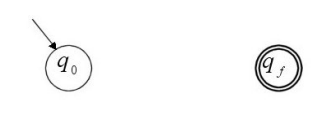
\includegraphics[scale=0.5]{imagenes/nothing}
  \end{center}
\end{figure}
\begin{figure}[H]
  \begin{center}
    \caption*{\(r=\lambda\)}
    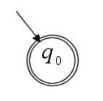
\includegraphics[scale=0.5]{imagenes/lambda}
  \end{center}
\end{figure}
\begin{figure}[H]
  \begin{center}
    \caption*{\(r=a\)}
    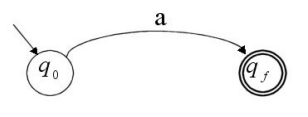
\includegraphics[scale=0.5]{imagenes/a}
  \end{center}
\end{figure}

\subsubsection{Pasos inductivos}
Sean \(r_1\) y \(r_2\) dos expresiones regulares. Supongamos que existen AFND-\(\lambda\) \\ \(M_1=\langle Q_1, \Sigma_1, \delta_1, q_1, \{f_1\}\rangle\) y \(M_2 =\langle Q_2, \Sigma_2, \delta_2, q_2, \{f_\}\rangle\) tal que \(\mathcal{L}(M_1) = \mathcal{L}(r_1)\) y \(\mathcal{L}(M_2) = \mathcal{L}(r_2)\). Vamos a armar a partir de estos autómata uno nuevo que acepte los lenguajes generados por las expresiones \(r_1|r_2\), \(r_1r_2\), \(r_1^*\) y \(r^+\).

\paragraph{\(\bm{r_1|r_2}\):} Podemos construir un automata \(M_0=\langle Q_0, \Sigma_0, \delta_0, q_0, \{f_0\}\rangle\) tal que \(\mathcal{L}(M_0) = \mathcal{L}(r_1|r_2)\) de la siguiente forma:
\begin{itemize}
  \item \(Q_0 = Q_1 \cup Q_2 \cup \{q_0, f_0\}\)
  \item \(\Sigma_0 = \Sigma_1 \cup \Sigma_2\)
  \item \(\delta_0: Q_0 \times \Sigma_0 \rightarrow \mathcal{P}(Q_0)\)
        \begin{itemize}
          \item[] \(\delta(q_0, \lambda) = \{q_1, q_2\}\)
          \item[] \(\delta(q, a) = \delta_1(q, a)\) para \(q\in Q_1-\{f_1\}\) y \(a\in \Sigma_1\cup\{\lambda\}\)
          \item[] \(\delta(q, a) = \delta_2(q, a)\) para \(q\in Q_2-\{f_2\}\) y \(a\in \Sigma_2\cup\{\lambda\}\)
          \item[] \(d(f_1,\lambda) = d(f_2,\lambda) = \{f_0\}\)
        \end{itemize}
\end{itemize}
\begin{figure}[H]
  \begin{center}
    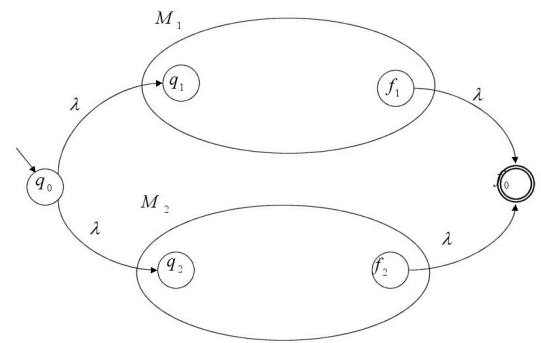
\includegraphics[scale=0.5]{imagenes/union}
  \end{center}
\end{figure}

\paragraph{\(\bm{r_1r_2}\):} \(M_0=\langle Q_0, \Sigma_0, \delta_0, q_1, \{f_2\}\rangle\):
\begin{itemize}
  \item \(Q_0 = Q_1 \cup Q_2\)
  \item \(\Sigma_0 = \Sigma_1 \cup \Sigma_2\)
  \item \(\delta_0: Q_0 \times \Sigma_0 \rightarrow \mathcal{P}(Q_0)\)
        \begin{itemize}
          \item[] \(\delta(q, a) = \delta_1(q, a)\) para \(q\in Q_1-\{f_1\}\) y \(a\in \Sigma_1\cup\{\lambda\}\)
          \item[] \(\delta(q, a) = \delta_2(q, a)\) para \(q\in Q_2-\{f_2\}\) y \(a\in \Sigma_2\cup\{\lambda\}\)
          \item[] \(d(f_1,\lambda) = \{q_2\}\)
        \end{itemize}
\end{itemize}
\begin{figure}[H]
  \begin{center}
    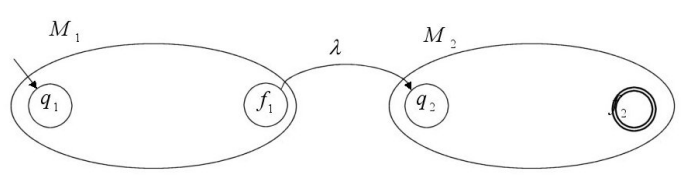
\includegraphics[scale=0.5]{imagenes/concat}
  \end{center}
\end{figure}

\paragraph{\(\bm{r_1^*}\):} \(M_0=\langle Q_0, \Sigma_1, \delta_0, q_0, \{f_0\}\rangle\):

\begin{itemize}
  \item \(Q_0 = Q_1 \cup \{f_0, q_0\}\)\
  \item \(\delta_1: Q_0 \times \Sigma_1 \rightarrow \mathcal{P}(Q_0)\)
        \begin{itemize}
          \item[] \(\delta(q_0, \lambda) = \delta(f_1,\lambda) = \{q_1, f_0\}\)
          \item[] \(\delta(q, a) = \delta_1(q, a)\) para \(q\in Q_1-\{f_1\}\) y \(a\in \Sigma_1\cup\{\lambda\}\)
        \end{itemize}
\end{itemize}
\begin{figure}[H]
  \begin{center}
    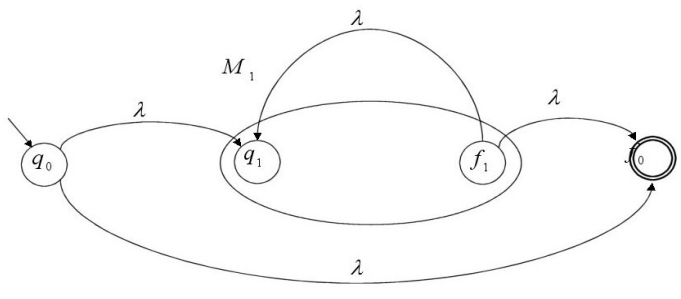
\includegraphics[scale=0.5]{imagenes/estrella}
  \end{center}
\end{figure}

Para el caso \(r_1^+\) es el mismo autómata que para este caso sin la transición \(q_0\overset{\lambda}{\rightarrow}f_0\).

\subsection{AFD a expresión regular}
\label{subsec:afd-er}
Dado un AFD \(M=\langle\{q_1, \dots, q_n\}, \Sigma, \delta, q_1, F\rangle\), que acepta el lenguaje \(\mathcal{L}\), existe una expresión regular que denota el mismo lenguaje.

\subsubsection{Demostración}
Nombremos \(R^k_{i,j}\) a la expresión regular cuyo lenguaje \(\omega \subseteq\Sigma^*\) son las cadenas que llevan al autómata \(M\) desde el estado \(q_i\) al estado \(q_j\) pasando solo por estados \(q_l\) con \(l\leq k\). En particular \(R^n_{i,j}\) es la expresión regular que representa todas las cadenas que permiten ir del estado \(i\) al estado \(j\).

Vamos a buscar como construir \(R^k_{i,j}\) para cada \(k\in\{0, \dots, n\}\) de manera inductiva. Suponiendo que demostramos la existencia de esta expresión regular, podemos concluir que la unión \(R^n_{1,f_1}|R^n_{1,f_2}|...|R^n_{1,f_m}\) (con \(f_1\dots f_m\in F\)) es la expresión regular que representa el lenguaje \(\mathcal{L}\):

\paragraph*{Caso base (\(k=0\)):} Como todos los estados están enumerados del 1 para arriba, \(k=0\) significa que no debe haber estados intermedios en el camino entre \(q_i\) y \(q_j\), por lo que pueden ser de dos formas:
\begin{itemize}
  \item Una arco del estado \(i\) al estado \(j\).
  \item Un camino de longitud cero que solo contiene el estado \(i\).
\end{itemize}

Si \(i\neq j\), entonces solo es posible la primera opción. Debemos examinar el AFD y encontrar aquellos simbolos que nos permitan ir del estado \(i\) al estado \(j\).

\begin{enumerate}
  \item Si no existe tal símbolo, entonces \(R^0_{i,j} = \varnothing\).
  \item Si existe exactamente un símbolo \(a\), entonces \(R^0_{i,j} = a\).
  \item Si existen más de un símbolo, entonces \(R^0_{i,j} = a_1|a_2|...|a_n\).
\end{enumerate}

Ahora, si \(i = j\) entonces los caminos de longitud cero también son posibles, por lo que habría que agregar a cada una de las expresiones recién mencionadas el simbolo \(\lambda\):
\begin{enumerate}
  \item \(R^0_{i,j} = \lambda\).
  \item \(R^0_{i,j} = a|\lambda\).
  \item \(R^0_{i,j} = a_1|a_2|...|a_n|\lambda\).
\end{enumerate}

\paragraph{Paso inductivo:} Supongamos que hay un camino desde el estado \(i\) al estado \(j\) que no pasa por estados mas grandes \(k\). Entonces podemos considerar las siguientes dos opciones:
\begin{enumerate}
  \item El camino no pasa por el estado \(k\), por lo que el lenguaje de \(R^{k-1}_{i,j}\) contiene a ese camino.
  \item El camino pasa por el estado \(k\) por lo menos una vez. Entonces podemos partir el camino en varias partes:
        \begin{figure}[H]
          \begin{center}
            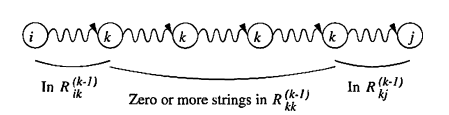
\includegraphics[scale=0.75]{imagenes/afd_regular.png}
          \end{center}
        \end{figure}
        La primer parte, va desde el estado \(i\) al estado \(k\) sin pasar por \(k\), la última parte es desde el estado \(k\) al estado \(j\) sin pasar por \(k\), y todas las partes intermedia s van desde el estado \(k\) al estado \(k\) sin pasar por \(k\). Cada una de estas partes ya tiene una expresión regular asociada: \(R^{k-1}_{i,k}\), \(R^{k-1}_{k,k}\), \(R^{k-1}_{k,j}\), por lo que podemos unirlas para obtener la expresión regular que representa el camino completo de la siguiente forma:
        \[
          R^{k-1}_{i,k}\left(R^{k-1}_{k,k}\right)^*R^{k-1}_{k,j}
        \]
\end{enumerate}

Entonces \(R^k_{i,j}\) es la unión de las expresiones de los dos tipos de caminos que acabamos de describir:
\[
  R^k_{i,j} = R^{k-1}_{i,j} \cup R^{k-1}_{i,k}\left(R^{k-1}_{k,k}\right)^*R^{k-1}_{k,j}
\]

Finalmente, si construimos en orden todas estas expresiones regulares desde \(R^0_{i,j}\), eventualmente llegaremos hasta \(R^n_{i,j}\).

Y como dijimos, más arriba si calculamos \(R^0_{1,j}\) para cada \(q_j\in F\) y unimos todas las expresiones, obtendremos la expresión regular que representa el lenguaje \(\mathcal{L}\).

\newpage
\subsection{Gramática regular a AFND}
Dada una grámatica regular \(G = \langle V_N, V_T, P, S\rangle\), podemos construir un AFND \\ \(M=\langle Q,\Sigma, \delta, q_0, F\rangle\) que reconozca el lenguaje generado por \(G\)

\subsubsection{Demostración}
Vamos a constuir el autómata finito no determinista \(M\) y demostrar que reconoce el lenguaje generado por \(G\).
\paragraph{Construcción de \(M\):} Construyamos \(M\) de la siguiente manera:
\begin{itemize}
  \item \(Q = V_N\cup\{q_f\}\). Denotarmeos \(q_A\) al estado que representa al no símbolo no terminar \(A\).
  \item \(\Sigma = V_T\)
  \item \(q_0 = q_S\)
  \item Si \(A, B \in V_N\) y \(a\in\Sigma\), entonces:
        \begin{itemize}
          \item \(q_B\in\delta(q_A, a) \iff A \rightarrow aB \in P\)
          \item \(q_f \in \delta(q_A, a) \iff A \rightarrow a \in P\)
          \item \(q_A\in F \iff A \rightarrow \lambda \in P\)
          \item \(q_f\in F\)
        \end{itemize}
\end{itemize}

\paragraph{Equivalencia clausura transitiva de producciones y \(\delta\): } Vamos a probar por inducción que
\[A   \deriva \alpha B \iff q_B\in\hat\delta(q_A, \alpha)\]

\begin{itemize}
  \item \textbf{Caso base \(\alpha = \lambda\):}
        \begin{itemize}
          \item \(A\deriva \alpha B\), pero las gramáticas regulares no acentan producciones que vayan de un no terminal a otro sin pasar por un terminal, por lo que \(B = A\). Osea \(A\deriva \alpha A\).
          \item Además, como es un AFND, no tiene transiciones lambda, osea que \(\delta(q_A, \lambda) = \{q_A\}\), por lo que \(q_A\in\hat\delta(q_A, \alpha)\).
        \end{itemize}
  \item \textbf{Caso inductivo \(\alpha = \beta a\):}
        \begin{align*}
          A\deriva \alpha B   \iff            & A\deriva \beta aB \iffa{def.} \red{\exists C\in V_N: A \deriva \beta C} \wedge \blue{C\rightarrow aB} \\
          \iffab{\red{H.I}}{\blue{constr. M}} & \blue{\exists q_C\in Q, q_c\in\hat\delta(q_A,\alpha)} \land \red{q_B\in\delta(q_C,a)}                 \\
          \iff                                & q_B\in \delta(\hat\delta(q_A,\alpha),a)                                                               \\
          \iff                                & q_B\in\hat\delta(q_A, \beta a) \iff q_B\in\hat\delta(q_A, \alpha)                                     \\
        \end{align*}
\end{itemize}

\paragraph{Demostración de la equivalencia:} Vamos a demostrar que el lenguaje generado por \(G\) y \(M\) son iguales, osea que \(\alpha a\in\mathcal{L}(M)\iff S\deriva \alpha a\).
Como \(G\) es una grámatica regular, hay solo dos formas de llegar desde \(S\) hasta \(\alpha a\):
\begin{enumerate}
  \item \(\exists A\in V_N: S \deriva \alpha A \wedge A \rightarrow a \in P\)
  \item \(\exists B\in V_N: S \deriva \alpha aB \wedge B \rightarrow \lambda \in P\)
\end{enumerate}
Entonces:

\begin{align*}
  S\deriva \alpha a \iffa{def. G} & (\exists A\in V_N: S \deriva \alpha A \wedge A \rightarrow a \in P)\lor(\exists B\in V_N: S \deriva \alpha aB \wedge B \rightarrow \lambda \in P)    \\
  \iffa{Equiv. anterior}          & (\exists q_A\in Q, q_A\in\hat\delta(q_0, \alpha) \land q_f\in\delta(q_A, a)) \lor (\exists q_B\in Q, q_B\in\hat\delta(q_0, \alpha a) \land q_B\in F) \\
  \iffa{def. \(\delta\)}          & q_f\in\delta(q_S, \alpha a) \lor (\exists q_B\in Q, q_B\in\hat\delta(q_0, \alpha a) \land q_B\in F)                                                  \\
  \iff                            & \alpha a \in \mathcal{L}(M)                                                                                                                          \\
\end{align*}

Falta ver que pasa si \(\lambda\in\mathcal{L}(G)\):

\[ \lambda\in\mathcal{L}(G) \iff S\deriva \lambda \iff S\rightarrow \lambda \in P \iff q_S\in F \iff \lambda \in \mathcal{L}(M)\]
\subsection{AFD a gramática regular}
Dado un AFD \(M=\langle Q, \Sigma, \delta, q_0, F\rangle\), existe una gramática regular \(G=\langle V_N, V_T, P, S\rangle\) equivalente

\subsubsection{Demonstración}
\paragraph{Contrucción de \(G\):} Vamos a construir \(G\) de la siguiente forma:
\begin{itemize}
  \item \(V_N = Q\), para mayor claridad llamamos \(A_p\) al no terminal correspondiente al estado \(p\in Q\)
  \item \(V_T = \Sigma\)
  \item \(S = q_0\)
  \item Si \(q\in Q \land q\notin F\) entonces \(A_p \rightarrow aA_q \in P \iff \delta(p,a) = q\)
  \item Si \(q\in F\) entonces \(A_p \rightarrow a \in P \iff \delta(p,a) = q\)
  \item \(S\rightarrow \lambda \in P \iff q_0\in F\)
\end{itemize}

\paragraph{Paso intermedio:} Vamos a demostrar por inducción: \[ \hat\delta(p,\alpha) = q \iff A_p \deriva \alpha A_q\]

\begin{itemize}
  \item \textbf{Caso base:} \(\alpha = \lambda\) es trivial:
        \begin{align*}
           & \hat\delta(p,\lambda) = q \iff A_p \deriva A_p
        \end{align*}
  \item \textbf{Caso inductivo \(\alpha = \beta a\):} Queremos probar que \(\hat\delta(p,\alpha) = q \iff A_p \deriva \alpha A_q\).

        Nuestra hipotesis inductiva: \(\hat\delta(p,\beta) = q \iff A_p \deriva \beta A_q\) para todo \(|\beta| \leq n\)

        \begin{align*}
           & \hat\delta(p, \alpha) = \hat\delta(p, \beta a) = q \iffa{def.}\blue{\exists r\in Q:~\hat\delta(p,\beta) = r} \land \red{\delta(r, a) = q}          \\
           & \iffab{\blue{H.I}}{\red{constr. G}} \blue{\exists A_r, A_p \deriva \beta A_r} \land \red{A_r \rightarrow a A_q \in P} \iff A_p \deriva \beta a A_q \\
        \end{align*}
\end{itemize}

\paragraph{Demostración de equivalencia de lenguajes:}
\begin{align*}
   & \alpha a\in\mathcal{L}(M) \iffa{def.} \hat\delta(q_0, \alpha a) \in F \iffa{def.} \exists q\in Q:~\hat\delta(q_0, \alpha) = q \land \delta(q,a)\in F \\
   & \underset{\text{paso intermedio}}{\iff} \exists A_p, A_{q0} \deriva \alpha A_p \land A_p \rightarrow a \in P \iff A_{q0} \deriva \alpha a            \\
   & \underset{\text{def.}}{\iff} \alpha a \in\mathcal{L}(G)
\end{align*}


\newpage
\section{Minimización de AFD}
\subsection{Indistinguibilidad}
Sea \(M=\langle Q, \Sigma, \delta, q_0, F\rangle\) un AFD, decimos que \(p,q\in Q\),  son indistinguibles \((p\equiv q)\) si para toda cadena \(\alpha\in\Sigma^*\) tal que \(\hat\delta(p,\alpha) \in F\) entonces pasa que \(\hat\delta(q,\alpha) \in F\) y viceversa. Si \(p, q\in Q\) son indistinguibles, entonces decimos que \(p\) y \(q\) son equivalentes.

\[ p \equiv q \iff \forall \alpha \in \Sigma^*:~(\hat\delta(p,\alpha) \in F \iff \hat\delta(q,\alpha) \in F)\]

\paragraph{Teorema:} Si \(p\) y \(q\) son indistinguibles, sea \(\alpha\in\Sigma^*\) entonces \(\hat\delta(p,\alpha) \equiv \hat\delta(q,\alpha)\)

\[ p \equiv q \implies \forall \alpha \in \Sigma^*:~\hat\delta(p,\alpha) \equiv \hat\delta(q,\alpha)\]
\begin{demo}[0.8\textwidth]
  Sean \(p,q\in Q\), \(p\equiv q\).

  Supogamos que existe \(\alpha\in\Sigma^*\) tal que \(\hat\delta(p, \alpha) \not\equiv \hat\delta(q,\alpha)\) entonces existe una cadena \(\gamma\in\Sigma^*\) que distingue a \(\hat\delta(p,\alpha)\) de \(\hat\delta(q,\alpha)\). Osea que \(\hat\delta(\hat\delta(p,\alpha), \gamma) \in F\) y \(\hat\delta(\hat\delta(q,\alpha), \gamma) \not\in F\) (o viceversa).

  Por def: \(\hat\delta(\hat\delta(p,\alpha),\gamma) = \hat\delta(p,\alpha\gamma)\) y \(\hat\delta(\hat\delta(q,\alpha), \gamma) = \hat\delta(p,\alpha\gamma)\). Entonces, como \(\alpha\gamma\) es una cadena que nos permite distinguir \(p\) de \(q\), es decir \(p \not\equiv q\). Absurdo.
\end{demo}

\paragraph{Teorema:} \(\equiv\) es una relación de equivalencia.

\begin{demo}[0.8\textwidth]
  \begin{itemize}
    \item \textbf{Reflexividad:} \(p\equiv p\):
          \[ \forall \alpha \in \Sigma^*:~(\hat\delta(p,\alpha) \in F \iff \hat\delta(p,\alpha) \in F) \iff p \equiv p \]
    \item \textbf{Simetría:} \(p\equiv q \implies q\equiv p\):
          \begin{align*}
             & p \equiv q \implies \forall \alpha \in \Sigma^*:~(\hat\delta(p,\alpha) \in F \iff \hat\delta(q,\alpha) \in F)  \\
             & \iff \forall \alpha \in \Sigma^*:~(\hat\delta(q,\alpha) \in F \iff \hat\delta(p,\alpha) \in F) \iff q \equiv p
          \end{align*}
    \item \textbf{Transitividad:} \(p\equiv q \land q\equiv r \implies p\equiv r\):
          \begin{itemize}
            \item[] \(p \equiv q \implies \forall \alpha \in \Sigma^*:~(\hat\delta(p,\alpha) \in F \iff \hat\delta(q,\alpha) \in F)\)
            \item[] \(q \equiv r \implies \forall \alpha \in \Sigma^*:~(\hat\delta(q,\alpha) \in F \iff \hat\delta(r,\alpha) \in F)\)
          \end{itemize}
          Entonces
          \begin{align*}
             & \forall \alpha \in \Sigma^*:~(\hat\delta(p,\alpha) \in F \iff \hat\delta(r,\alpha) \in F) \iff p \equiv r
          \end{align*}
  \end{itemize}
\end{demo}

\subsubsection{Indestinguibilidad de orden k}
\[ p \overset{k}{\equiv} q \iff \forall \alpha\in\Sigma^*, (|\alpha|\leq k) \implies (\hat\delta(p,\alpha) \in F \iff \hat\delta(q,\alpha) \in F)\]

\paragraph{Propiedades:}
\begin{enumerate}
  \item \(\overset{k}{\equiv}\) es un relación de equivalencia.
        \begin{demo}[0.8\textwidth]
          Es exactamente igual a la demostración \(\equiv\) es transitiva.
        \end{demo}
  \item \(\overset{k+1}{\equiv}\subseteq\overset{k}{\equiv}\)
        \begin{demo}[0.8\textwidth]
          \[ p \overset{k+1}{\equiv} q \implies \forall \alpha\in\Sigma^*, (|\alpha|\leq k+1) \implies (\hat\delta(p,\alpha) \in F \iff \hat\delta(q,\alpha) \in F)\]

          Ahora como esto vale \(\forall \alpha\in\Sigma^*, (|\alpha|\leq k+1)\), necesarimente vale \(\forall \alpha\in\Sigma^*, (|\alpha|\leq k)\). Entonces
          \[ \forall \alpha\in\Sigma^*, (|\alpha|\leq k+1) \implies (\hat\delta(p,\alpha) \in F \iff \hat\delta(q,\alpha) \in F) \implies p \overset{k}{\equiv} q\]
        \end{demo}
  \item \(\left(Q / \overset{0}{\equiv}\right) = \{Q-F, F\}\) si \(Q - F \neq \emptyset\) y \(F \neq\emptyset\). En castellano, \(\overset{0}{\equiv}\) divide al conjunto de estados en estados finales y no finales.
  \item \(
        p\overset{k+1}{\equiv} q \iff \left(p \overset{0}{\equiv} q
        \right) \land \left(
        \forall a\in\Sigma, \delta(p,a) \overset{k}{\equiv} \delta(q,a)
        \right)
        \)
        \begin{demo}[0.8\textwidth]
          \begin{itemize}
            \item[\(\Rightarrow)\)] Como \(\overset{k+1}{\equiv} \subseteq \overset{k}{\equiv}\) entonces \( p\overset{k+1}{\equiv} q \implies p \overset{0}{\equiv} q\).

              Por otro lado, supongamos que no vale \(\left(
              \forall a\in\Sigma, \delta(p,a) \overset{k}{\equiv} \delta(q,a)
              \right)\) entonces
              \[
                \exists a\in\Sigma,~\exists\alpha\in\Sigma^*, (|\alpha|\leq k) \land \hat\delta(\delta(p,a), \alpha) \in F \land \hat\delta(\delta(q,a),\alpha) \notin F
              \]

              o viceversa. Pero entonces \( p \overset{k+1}{\not\equiv} q\) ya que \(a\alpha\leq k + 1 \) y \(a\alpha\) distinque a \(p\) y a \(q\).
          \end{itemize}
        \end{demo}
        \begin{demoPart}[0.8\textwidth]
          \begin{itemize}
            \item[\(\Leftarrow )\)] Supogamos que \(p \overset{k}{\equiv} q\). Entonces ó \(p \overset{0}{\equiv} q\) ó \(\exists a\alpha,~|a\alpha| \leq k + 1\) que distingue \(p\) de \(q\), o sea que:
              \[
                \hat\delta(\delta(p,a),\alpha)\in F \land \hat\delta(\delta(q,a),\alpha)\notin F
              \]

              o viceversa. Pero entonce \(\delta(p,a) \overset{k+1}{\not\equiv} \delta(q,a)\).
          \end{itemize}
        \end{demoPart}
  \item \(\left(\overset{k+1}{\equiv} = \overset{k}{\equiv}\right) \implies \forall n\geq 0, \left(
        \overset{k+n}{\equiv} = \overset{k}{\equiv}
        \right)
        \)
        \begin{demo}[0.8\textwidth]
          Lo vamos a demostrar por inducción:
          \begin{itemize}
            \item[] \textbf{Caso base:}\(n=0\). Entonces \(k \overset{k}{\equiv}=\overset{k}{\equiv}\).
            \item[] \textbf{Paso inductivo:} Suponemos que es cierto para \(n\), osea que vale \(\overset{k+1}{\equiv} =\overset{k}{\equiv} \implies \overset{k+n}{\equiv} = \overset{k}{\equiv}\)

              Queremos probar \(\overset{k+1}{\equiv} =\overset{k}{\equiv} \implies \overset{k+n+1}{\equiv} = \overset{k}{\equiv}\):

              Sabemos que \(\overset{k+n+1}{\equiv} = \overset{k}{\equiv}\) si y solo si \(\forall p,q\in Q, \left(
              p\overset{k}{\equiv} q \iff p\overset{k+n+1}{\equiv} q
              \right)\)

              Por la propiedad (4), tenemos:
              \begin{align*}
                p\overset{k+n+1}{\equiv} \iff       & \left(p \overset{0}{\equiv}q\right)\land\left(
                \forall a\in\Sigma, \delta(p,a) \overset{k+n}{\equiv} \delta(q,a)
                \right)   \left(p \overset{0}{\equiv}q\right)                                                                                                           \\ &\land\left(
                \forall a\in\Sigma, \delta(p,a) \overset{k+n}{\equiv} \delta(q,a)
                \right)                                                                                                                                                 \\
                \underset{\text{prop. 2}}{\implies} & \left(p \overset{0}{\equiv}q\right)\land\left(
                \forall a\in\Sigma, \delta(p,a) \overset{k}{\equiv} \delta(q,a) \right)                                                                                 \\
                                                    & \underset{\text{prop. 4}}{\implies} p \overset{k+1}{\equiv}q \underset{\text{prop. 2}}{\implies} q \overset{k}{p}
              \end{align*}
          \end{itemize}
        \end{demo}
\end{enumerate}
\subsection{Autómatas finito determinístico mínimo}
Sea \(M=\langle Q, \Sigma, \delta, q_0, F\rangle\) un AFD sin estados inaccesibles, el AFD mínimo equivalente \(M'= \langle Q', \Sigma, \delta', q_0, F'\rangle\) se define de la siguiente manera:
\begin{itemize}
  \item \(Q' = Q / \equiv\). Vamos a notar \([q]\) al estado que representa a la clase de equivalencia que contiene a \(q\).
  \item \(\delta'([q], a) = [\delta(q,a)]\)
  \item \(q_0' = [q_0]\)
  \item \(F' = \{[q]\in Q'~:~ q \in F\}\)
\end{itemize}

\paragraph{Teorema:}
\[\forall \alpha\in\Sigma^*, \hat\delta(q, \alpha) = r \implies \hat\delta'(q_0', \alpha) = \hat\delta'([q], \alpha) = [r]\]

\begin{demo}[0.8\textwidth]
  Va a ser por inducción en la longitud de \(\alpha\):
  \begin{itemize}
    \item \(\alpha = \lambda\): \(\hat\delta(q, \epsilon) = q\), por def. de \(\hat\delta\)

          \(\hat\delta'(q_0', \epsilon) = \hat\delta'([q], \epsilon) = [q]\) por def. de \(\hat\delta'\)

          Entonces \(\hat\delta(q, \lambda) = q \implies \hat\delta'([q], \lambda) = [q]\)
    \item Paso inductivo: Sea \(\alpha = \beta a\), queremos probar que \(\hat\delta(q,\alpha) = r \implies \hat\delta'([q], \alpha) = [r]\).

          Nuestra hipotesis inductiva es \(\forall \beta\in\Sigma^*,~|\beta|\leq n,~\hat\delta(q, \beta) = p \implies \hat\delta'([q], \beta) = [p]\)

          Entonces:

          \[ \hat\delta(q, \alpha) = \hat\delta(q, \beta a) = \delta(\hat\delta(q, \beta), a) = \hat\delta(p, a) = r \underbrace{\implies}_{\text{constr. }\delta'} \delta'([p], a) = [r] ~(1)\]

          Además, por hipotesis inductiva sabemos que \(\hat\delta'([q], \beta) = [p]\), entonces remplazando en el último término de la ecuación (1) obtenemos:

          \[ \delta'([p], \alpha) = \delta'(\hat\delta'([q], \beta), a) = \hat\delta(q,\beta a) = \hat\delta(q,\alpha) = [r] \]
  \end{itemize}

\end{demo}
\subsection{Algoritmo de minimización de un AFD}
\begin{algorithmic}
  \Require \(M = \langle Q, \Sigma, \delta, q_0, F\rangle\)
  \State \(P\leftarrow\{Q-F, F\}\) \Comment{\(P = \overset{0}{\equiv}\), separamos los estados finales de los no finales}
  \State \(stop\leftarrow false\)
  \While{\(stop = false\)}
  \State\(P'\leftarrow\emptyset\)
  \For{\(X\in P\)} \Comment{Separamos cada clase de equivalencia en las subclases de \(\overset{n+1}{\equiv}\)}
  \While{\(\exists e\in X : \lnot\texttt{marked}(e, X)\)} \Comment{Elegimos un nuevo representante para cada clase}
  \State\(X_1\leftarrow\{e\}\)
  \State\(\texttt{marked}(e,X)\)
  \For{\(e'\in X: e\neq e'\)} \Comment{Conseguimos los elementos de esa clase}
  \If{\(\lnot\texttt{marked}(e', X)\land(\forall a\in\Sigma,~[\delta(e,a)] = [\delta(e',a)])\)}
  \State\(X_1\leftarrow X_1\cup\{e'\}\)
  \State\(\texttt{mark}(e',X)\)
  \EndIf
  \EndFor
  \State \(P'\leftarrow P'\cup \{X_1\}\)
  \EndWhile
  \EndFor
  \If{\(P \neq P'\)}
  \State \(P\leftarrow P'\)
  \Else
  \State \(stop\leftarrow true\)
  \EndIf
  \EndWhile
\end{algorithmic}

\paragraph{Lema:} Sean \(M=\langle Q, \Sigma, \delta, q_0, F\rangle\) y \(M'=\langle Q', \Sigma, \delta', q'_0, F'\rangle\) dos AFDs. Si \(M\) no poseee estados inaccesibles y todo par de cadenas que conducen a estados diferentes de \(M\) conducen a estados diferentes de \(M'\), entonces la cantidad de estados de \(M'\) es mayor o igual a la cantidad de estados de \(M\). Es decir:

\[
  \left(
  \forall\alpha,\beta\in\Sigma^*,~\hat\delta(q, \alpha) \neq \hat\delta(q, \beta) \implies \hat\delta'(q_0', \alpha) \neq \hat\delta'(q_0', \beta)
  \right) \implies |Q|\leq |Q'|
\]

\begin{demo}[0.8\textwidth]
  Sea \(g:Q\to\Sigma^*\) definida por \(g(q) = \min\left\{\alpha\in\Sigma^*:~\hat\delta(q_0,\alpha) = q\right\}\) donde suponemos una relación de orden en \(\Sigma^*\) dada por la longitud para cadenas de distinta longitud, y por el lexicográfico para las cadenas de igual longitud. Definamos \(f: Q\to Q'\) con \(f(q)=\hat\delta'(q_0', g(q))\).

  Como para cualquier par de estados diferentes \(p,q\in Q\) es cierto que \(\hat\delta(q_0, g(p))\neq\hat\delta(q_0, g(q))\), entonces \(\hat\delta'(q_0', g(p))\neq\hat\delta'(q_0', g(q))\). Lo que equivale a decir que \(f(p)\neq f(q)\). Por lo tanto, \(f\) es una función inyectiva, es decir que \(|Q|\leq |Q'|\).
\end{demo}

\paragraph{Lema:} Sea \(M_R = \langle Q_R, \Sigma, \delta_R, q_{R0}, F_R\rangle\) el autómata reducido correspondiente a \\ \(M = \langle Q, \Sigma, \delta, q_0, F\rangle\). Entonces, cualquier autómata \(M' = \langle Q', \Sigma, \delta', q_{0'}, F'\rangle\) que reconozca el mismo lenguaje que \(M\) no poseerá menos estados que \(M_R\). Osea:
\[
  \forall M',~\mathcal{L} (M') = \mathcal{L} (M) \implies |Q'| \geq |Q_R|
\]

\begin{demo}[0.8\textwidth]
  Supongamos que \(\exists M'\) tal que \( |Q'| < |Q_R|\), entonces según el lema anterior deben existir dos cadenas \(\alpha,\beta\in\Sigma^*\) tales que
  \[
    \hat{\delta_R}(q_0,\alpha) \neq \hat{\delta_R}(q_0,\beta) \land \hat{\delta'}(q_0',\alpha) = \hat{\delta'}(q_0',\beta)
  \]
  Pero entonces, como \(\hat{\delta_R}(q_0,\alpha)\) y \(\hat{\delta_R}(q_0,\beta)\) son estados diferentes, entonces \(\hat{\delta}(q_0,\alpha)\) y \(\hat{\delta}(q_0,\beta)\) son estados distinguibles por pertenecer al autómata reducido \(M_R\) entonces \(\exists\gamma\in\Sigma^*\) tal que:
  \[
    \hat{\delta}(q_0,\alpha\gamma)\in F \land \hat{\delta}(q_0,\beta\gamma)\notin F
  \]
  o viceversa. Entonces \(\alpha\gamma\in\mathcal{L}(M_R) \iff \beta\gamma\notin\mathcal{L}(M_R)\).

  Por otro lado, como \(\hat\delta'(q_0',\alpha) = \hat\delta'(q_0',\beta)\), es obvio que \[
    \hat\delta'(q_0',\alpha\gamma)\in F\land \hat\delta'(q_0',\beta\gamma)\in F
  \] o ninguno de los dos perteneces a \(F\). De esto se inifiere que \(\alpha\gamma\in\mathcal{L}(M') \iff \beta\gamma\in\mathcal{L}(M')\).

  Pero entonces, \(\mathcal{L}(M') \neq \mathcal{L}(M)\), se contradice nuestra hipotesis inicial.
\end{demo}

\newpage
\section{Lenguajes regulares}
\label{sec:pumping}
\subsection{Lema de pumping}
\label{subsec:pumping}
\paragraph{Propiedad:} Sea \(\mathcal{L}\) un lenguaje regular, si las longitudes de las cadenas de un lenguaje \(\mathcal{L}\) están acotadas superiormente, entonces \(\mathcal{L}\) tiene que ser finito.

\paragraph{Propiedad:} Si \(\mathcal{L}\) es un luenguaje regular infinito, entonces el grafo de un autómata fínito que acepte \(\mathcal{L}\) tiene que tener un camino desde el estado inicial hasta algún estado final que paso por algún ciclo.

\paragraph{Lema de pumping:} Sea \(\mathcal{L}\) un lenguaje regular, si \(\mathcal{L}\) es infinito, entonces todas las cadenas \(\omega\) de longitud mayor o igual a \(n\) (para algún \(n > 1\)) van a ser de la forma \(\omega=xy^iz\), es decir hay una parte de \(\omega\) que se repite \(i\) cantidad de veces:

\begin{align*}
   & \mathcal{L} \text{ es regular e infinito}\implies \exists n\in\mathbb{N}\text{ tal que } \\ &\forall\omega\in\mathcal{L},~|\omega|\geq n:\left( \exists x,y,z\in\Sigma^*: \omega=xyz\land|xy|\leq n\land|z|\geq 1 \land (\forall i\geq  0 :~ xy^iz\in\mathcal{L}\right) \\
\end{align*}
\begin{demo}[0.8\textwidth]  Supongamos que \(\mathcal{L}\) es un lenguaje regular. Entonces existe una AFD \(A =\langle Q, \Sigma, \delta, q_0, F\rangle\) que acepta \(\mathcal{L}\).

  Sea \(n = |Q|\) la cantidad de estados de \(A\) y \(\omega=a_1a_2\dots a_m\in\Sigma^*\) de longitud \(m > n\). Para cada \(i = 0,\dots, m\) definamos el estado \(p_i = \hat\delta(q_0, a_1\dots a_i)\) (el estado en el que se encuentra \(A\) después de haber consumido los primeros \(i\) símbolos de \(\omega\).

  Como el \(A\) solo tiene \(n\) estados pero hay \(m > n\) estados \(p_i\), es imposible que todos sean distintos. Por lo tanto, existen \(0 \leq i < j \leq n\) tales que \(p_i = p_j\).

  Considerar entonces la siguiente descomposición para \(\omega = xyz\):
  \begin{itemize}
    \item[] \(x = a_1\dots a_i\)
    \item[] \(y = a_{i+1}\dots a_j\)
    \item[] \(z = a_{j+1}\dots a_m\)
  \end{itemize}
  Entonces podemos concluir que:
  \begin{itemize}
    \item[] \(\hat\delta(q_0, x) = p_i\)
    \item[] \(\hat\delta(p_i, y) = p_j\) (que como son el mismo estado implica que \(A\) tiene un ciclo)
    \item[] \(\hat\delta(p_j, z) = p_m\)
  \end{itemize}

\end{demo}
\begin{demoPart}[0.8\textwidth]

  Observar que \(x\) podría ser la cadena vacía cuando \(i = 0\), \(z\) podría ser vacía si \(j = n = m\), pero \(y\) no puede ser vacía ya que se tomó \(i < j\).

  Vimos entonces que si \(\mathcal{L}\) es regular y \(|\omega| \geq n\) entonces podemos dividirla en cadenas \(x,y,z\) tal que \(|xy|\leq n\) y \(|z|\geq 1\). Ahora vamos a ver que si \(xyz \in \mathcal{L}\) entonces \(xy^kz \in \mathcal{L}\) para todo \(k\geq 0\).

  \begin{itemize}
    \item Si \(k = 0\) entonces \(xy^0z = xz\):
          \[\hat\delta(q_0, xz) = \hat\delta(\hat\delta(q_0, x), z) = \hat\delta(p_i, z) = \hat\delta(p_j, z) = p_m\]
          Y \(p_m\) es un estado final pues es el mismo estado al que llegamos si la entrada fuese \(xyz\in\mathcal{L}\). Entonces \(xz = xy^0z \in \mathcal{L}\).
    \item Si \(i > 0\). Entonces \(A\) consume \(x\) desde \(q_0\) y llega hasta \(p_i\). Luego \(A\) consume \(y\) desde \(p_i\) y llega hasta \(p_j\) (que son iguales) y repite este ciclo \(k\) veces hasta consumir todas las apariciones de \(y\) en la cadena. Finalmente \(A\) consume \(z\) desde \(p_j\) y llega hasta \(p_m\). Entonces \(A\) llega a un estado final y por lo tanto \(xy^kz \in \mathcal{L}\).
  \end{itemize}
\end{demoPart}
\paragraph{Contrarecíproco:}
\begin{align*}
   & \forall   n\in\mathbb{N}~\exists\omega\in\mathcal{L}\text{ tal que } |\omega|\geq n \land  \forall x,y,z\in\Sigma^*: \omega\neq xyz \lor|xy|\geq n\lor|z|\leq 1 \lor \exists i\geq 0,~ xy^iz\notin\mathcal{L} \\ &
  \implies \mathcal{L}\text{  no es regular}                                                                                                                                                                       \\
\end{align*}

\subsection{Operaciones sobre lenguajes regulares}
\subsubsection{Unión de lenguajes regulares}
Dados \(M_1\) y \(M_2\) AFDs que aceptan los lenguajes \(L_1\) y \(L_2\), respectivamente, podemos construir un AFD \(M = \langle Q_{\cup}, \Sigma, \delta_{\cup}, q_{0\cup}, F_{\cup}\rangle\) que acepte el lenguaje \(L_1 \cup L_2\) con:
\begin{itemize}
  \item \(Q_{\cup} = Q_1 \times Q_2\)
  \item \(\delta_{\cup}((q,r), a) = (\delta_1(q,a),\delta_2(r,a)) \) para \(q\in Q_1\), \(r\in Q_2\) y \(a\in\Sigma\)
  \item \(q_{0\cup} = (q_{0_1},q_{0_2})\)
  \item \(F_{\cup} = \{(q,r)\in Q_{\cup} \mid q\in F_1 \lor r\in F_2\}\)
\end{itemize}
\begin{demo}[0.8\textwidth]
  \begin{align*}
    \alpha\in\mathcal{L}(M_\cup) \iff & \hat\delta_\cup((q_{0_1}, q_{0_2}), \alpha) \in F_\cup \iff (\hat\delta_1(q_{0_1}, \alpha), \hat\delta_2(q_{0_2}, \alpha)) \in F_\cup \\ \iff &\hat\delta_1(q_{0_1}, \alpha) \in F_1 \lor \hat\delta_2(q_{0_2}, \alpha) \in F_2 \\
    \iff                              & \alpha\in\mathcal{L}(M_1) \lor \alpha\in\mathcal{L}(M_2)
  \end{align*}
\end{demo}

\subsubsection{Intersección de lenguajes regulares}
Dados \(M_1\) y \(M_2\) AFDs que aceptan los lenguajes \(L_1\) y \(L_2\), respectivamente, podemos construir un AFD \(M_\cap = \langle Q_{\cap}, \Sigma, \delta_{\cap}, q_{0\cap}, F_{\cap}\rangle\) que acepte el lenguaje \(L_1 \cap L_2\) con:
\begin{itemize}
  \item \(Q_{\cap} = Q_1 \times Q_2\)
  \item \(\delta_{\cap}((q,r), a) = (\delta_1(q,a),\delta_2(r,a)) \) para \(q\in Q_1\), \(r\in Q_2\) y \(a\in\Sigma\)
  \item \(q_{0\cap} = (q_{0_1},q_{0_2})\)
  \item \(F_{\cap} = \{(q,r)\in Q_{\cap} \mid q\in F_1 \land r\in F_2\}\)
\end{itemize}

\begin{demo}[0.8\textwidth]
  \begin{align*}
    \alpha\in\mathcal{L}(M_\cap) \iff & \hat\delta_\cap((q_{0_1}, q_{0_2}), \alpha) \in F_\cap \iff (\hat\delta_1(q_{0_1}, \alpha), \hat\delta_2(q_{0_2}, \alpha)) \in F_\cap \\ \iff &\hat\delta_1(q_{0_1}, \alpha) \in F_1 \land \hat\delta_2(q_{0_2}, \alpha) \in F_2 \\ \iff & \alpha\in\mathcal{L}(M_1) \land \alpha\in\mathcal{L}(M_2)
  \end{align*}
\end{demo}

\subsubsection{Complemento de lenguajes regulares}
\begin{teorema}
  El conjunto de lenguajes regulares incluido en \(\Sigma^*\) es cerrado respecto de la complementación. Es decir, si \(L\in\mathcal{L}(\Sigma^*)\) es un lenguaje regular entonces \(\bar{L}\in\mathcal{L}(\Sigma^*)\) también lo es.
\end{teorema}
\begin{demo}[0.8\textwidth]
  Sea \(\mathcal{L} = \mathcal{L}(M)\) con \(M=(Q,\Sigma,\delta,q_0,F)\) un AFD cuya función de transición \(\delta\) está definida para todos los elementos del alfabeto \(\Sigma\). Si hay algún símbolo \(a\in\Sigma\) que falta en las posibles transiciones desde un estado \(q\in Q\) entonces se puede agregar un estado trampa \(q_{trampa}\) (no final) y una transición \(\delta(q,a) = q_{trampa}\) para completar la definición de la función.

  Si armamos el automáta \(M_{\lnot} =\langle Q,\Sigma,\delta,q_0,Q - F\rangle\), entnonces \(\alpha\in\mathcal{L}M_{\lnot} \iff \delta(q_0, w) \in Q - F \iff \alpha\in\Sigma^* - L\).
\end{demo}

\begin{teorema}
  El conjunto de lenguajes regulares es cerrado respecto de la intersección
\end{teorema}

\begin{demo}[0.8\textwidth]
  Como ya probamos que el conjunto de lenguajes regulares es cerrado respecto de la unión y el complemento entonces si logramos escribir la interesección como combinación de estas dos operaciones podremos decir que también es cerrada respecto de la intersección:
  \[
    L_1 \cap L_2 = \overline{\overline{L_1\cap L_2}} = \overline{\overline{L_1} \cup \overline{L_2}}
  \]
\end{demo}
\begin{demoPart}[0.8\textwidth]
  Entonces si \(L_1\) y \(L_2\) son lenguajes regulares, entonces sus complementos también lo son y la unión de los complementos y el complemento de la misma también lo son.
\end{demoPart}

\begin{teorema}
  De estos ultimos tres teoremas puede deducirse que la unión finita y la intersección finita de lenguajes regulares dan por resultado un lenguaje regular.

  \[
    \forall n\in\mathbb{N},~\bigcup_{i=1}^n L_i \text{ es regular}
  \]
  \[
    \forall n\in\mathbb{N},~\bigcap_{i=1}^n L_i \text{ es regular}
  \]
\end{teorema}

\begin{demo}[0.8\textwidth]
  Por inducción sobre n:
  \begin{itemize}
    \item[] \textbf{Caso base:} \(n=0\). \[
        \bigcup_{i=1}^0 L_i = \emptyset \text{ es regular}
      \]
      \[ \bigcap_{i=1}^0 L_i  = \emptyset \text{ es regular}\]
    \item \textbf{Caso inductivo:} \(n\geq 1\). Supongamos que \(L_1,\dots,L_n\) son lenguajes regulares y que \(\overset{n-1}{\underset{i=1}{\bigcup}} L_i\) y \(\overset{n-1}{\underset{i=1}{\bigcap}} L_i\) son lenguajes regulares. Entonces:

          \[ \bigcup_{i=1}^{n} L_i = \bigcup_{i=1}^{n-1} L_i \cup L_n \text{ es regular}\]
          \[ \bigcap_{i=1}^{n} L_i = \bigcap_{i=1}^{n-1} L_i \cap L_n \text{ es regular}\]
  \end{itemize}
\end{demo}
\begin{teorema}
  Todo lenguaje finito es regular
\end{teorema}
\begin{demo}[0.8\textwidth]
  Sea \(L\) un lenguaje finito tal que \(|L| = n\) y \(x_i \in L\) con \(1 \leq i \leq n\).

  Entonces podemos definir \(n\) lenguajes \(L_i = \{ x_i \} \) regulares. Por el teorema anterior, la unión finita de lenguajes regulares es un lenguaje regular. Entonces \(L = \overset{n}{\underset{i=1}{\bigcup}} L_i\) es un lenguaje regular.
\end{demo}

\newpage
\subsection{Problemas decicibles acerca de lenguajes regulares}
\begin{enumerate}
  \item \textbf{Pertenencia:} Dado un lenguaje regular \(L\) y una cadena \(w\), determinar si \(w\in L\).
        \begin{itemize}
          \item[] Se construye un AFD \(M\) que reconozca \(L\) y se verifica si \(w\) es aceptada por \(M\).
        \end{itemize}
  \item \textbf{Finitud:} Dado un lenguaje regular \(L\), determinar si \(L\) es finito.
        \begin{itemize}
          \item[] Un lenguaje regular \(L\) es finito, si en su AFD ningún ciclo que es alcanzable desde el estado inicial puede, a su ve, alcanzar algún estado final.
            \[
              L \text{ finito } \iff \left(
              \forall q \in Q,\left(
                q_0 \deriva q \land q \deriva f \in F \implies \left(\not\exists q\overset{+}{\rightarrow} q\right)
                \right)
              \right)\]
            Escrito en función de \(\delta\):
            \begin{align*}
              L \text{ finito si y solo si: } \forall q \in Q & \text{ tal que } \left(
              \exists\alpha,\omega\in\Sigma^*,~\hat\delta(q_0, \alpha) = q \land \hat\delta(q, \omega) = f \in F
              \right)                                                                   \\ &\text{vale que} \left(\not\exists\beta\in\Sigma^+,~\hat\delta(q, \beta) = q\right)
            \end{align*}
        \end{itemize}
  \item \textbf{Vacuidad:} Dado un lenguaje regular \(L\), determinar si \(L\) es vacío.
        \begin{itemize}
          \item[] Se construye el AFD \(M\) que reconozca \(L\) y se verifica si el conjunto \(A\) de estados alcanzables de \(M\) tiene un estado final. Si \(F\cap A = \emptyset\), entonces \(L\) es vacío.
        \end{itemize}
  \item \textbf{Equivalencia:} Dados dos lenguajes regulares \(L_1\) y \(L_2\), determinar si \(L_1\) y \(L_2\) son equivalentes.
        \begin{itemize}
          \item[] Si el lenguaje \( (L_1 \cap \overline{L_2}) \cup (\overline{L_1}\cap L_2) \) es vacío, entonces \(L_1\) y \(L_2\) son equivalentes, si no no lo son.
        \end{itemize}
\end{enumerate}


\newpage
\section{Autómatas de Pila}
\label{sec:automatas-pila}

Los autómatas de pila (AP) son autómatas fínitos que además tienen la cpaidad de almacenar información en una pila con dos operaciones básicas: apilar y desapilar. La operación apilar consiste en agregar un elemento a la pila, mientras que la operación desapilar consiste en eliminar el elemento que se encuentra en la cima de la misma.

Cuando se va a realiar una transición, se consume un elemento de la cadena de entrada y un elemento del tope de la pila. Al moverse al  nuevo estado, el automáta puushea (apila) una cadena de símbolos en la pila (que puede ser vacía).

\paragraph{Definición:} Un autómata de pila (AP) es una 7-tupla $M = (Q, \Sigma, \Gamma, \delta, q_0, Z_0, F)$ donde:

\begin{itemize}
  \item $Q$ es un conjunto finito de estados.
  \item $\Sigma$ es el alfabeto de entrada y es finito.
  \item $\Gamma$ es un alfabeto de la pila y es finito.
  \item $\delta$ es la función de transición, que es un conjunto de reglas de la forma:
        \[ \delta: Q \times (\Sigma\cup\{\lambda\}) \times \Gamma \rightarrow \mathcal{P}(Q\times\Gamma^*) \]
        \[ \delta(q, a, Z) = \{ (p_1, \gamma_1), (p_2, \gamma_2), \ldots, (p_n, \gamma_n) \} \]
        \(\delta\) indica el estado que \(p_i\) al que se transiciona y la cadena \(\gamma_i\) que se apila en la pila.
  \item $q_0 \in Q$ es el estado inicial.
  \item $Z_0 \in \Gamma$ es el símbolo inicial de la pila.
  \item $F\subseteq Q$ es el conjunto de estados finales.
\end{itemize}

\subsection{Configuración instantanea}
\label{subsec:configuracion-instantanea}

Una configuración instantánea de un autómata de pila es una 3-tupla $(q, w, \gamma) \in Q\times\Sigma\times\Gamma^*$ donde:
\begin{itemize}
  \item $q \in Q$ es el estado actual.
  \item $w \in \Sigma^*$ es la parte de la cadena de entrada que no ha sido consumida.
  \item $\gamma \in \Gamma^*$ es el contenido de la pila.
\end{itemize}

La configuracion inicial de un automáta será entonces $\sigma = (q_0, \alpha, Z_0)$ si \(\alpha\) es la cadena que usamos de entrada.

\paragraph{Cambio de configuración:} Sea $M=\langle Q, \Sigma, \Gamma, \delta, q_0, Z_0, F \rangle$ un automáta de pila, \(a\in\Sigma\), \(\alpha\in\Sigma^*\), \(t\in\Gamma\), \(\tau,\pi\in\Sigma^*\) y \(q,r\in Q\). Definimos las transiciones \((\vdash\)) entre dos configuraciones instantaneas de la siguiente manera:
\begin{itemize}
  \item \((q, a\alpha, t\pi)\vdash (r, \alpha, \tau\pi)\) si \((r,\tau)\in\delta(q,a,t)\).
  \item \((q,   \alpha, t\pi)\vdash (r, \alpha, \tau\pi)\) si \((r,\tau)\in\delta(q,\lambda,t)\).
\end{itemize}

\subsection{Lenguajes reconocidos por un autómata}
\subsection{Lenguaje aceptado por estado final}
Son todas las cadenas \(\alpha\in\Sigma^*\) que hacen que el automáta llegue a un estado final \(q\in F\).

\[ \mathcal{L}(M) = \{ \alpha \in \Sigma^* \mid \exists q \in F \text{ tal que } (q_0, \alpha, Z_0) \overset{*}{\vdash}  (q, \lambda, Z_0) \} \]

\subsubsection{Lenguaje aceptado por pila vacía}
Son todas las cadenas \(\alpha\in\Sigma^*\) que hacen que el automáta llegue a un estado en el cual la pila quede vacía.

\[ \mathcal{L}_\lambda(M) = \{ \alpha \in \Sigma^* \mid \exists q \in F \text{ tal que } (q_0, \alpha, Z_0) \overset{*}{\vdash}  (q, \lambda, \lambda) \} \]


\begin{teorema}
  \label{teo:automata-pila}
  Sea \(M=\langle Q, \Sigma, \Gamma, \delta, q_0, Z_0, F \rangle\) un automáta que acepta el lenguaje \(\mathcal{L}(M)\) por estado final, entonces existe \(M'=\langle Q', \Sigma, \Gamma', \delta', q'_0, X_0, \emptyset \rangle\) tal que \(\mathcal{L}_\lambda(M') = \mathcal{L}(M)\).
\end{teorema}
\begin{demo}[0.8\textwidth]
  Construimos \(M'\) de la siguiente manera:
  \begin{itemize}
    \item \(Q' = Q \cup \{q_\lambda, q_0'\}\)
    \item \(\Gamma' = \Gamma \cup \{ X_0 \}\)
    \item \(\delta': Q'\times\Sigma\times\Gamma' \rightarrow \mathcal{P}(Q'\times\Gamma')\)
          \begin{enumerate}
            \item\(\delta'(q_0', \lambda, X_0) = \{ (q_0, Z_0X_0) \}\)
            \begin{itemize}
              \item[] \(M'\) entra al estado inicial de \(M\) con la pila \(Z_0X_0\). como \(X_0\) no es un símbolo de la pila de \(M\), \(M\) no puede vaciar la pila.
            \end{itemize}
            \item  \(\forall q\in Q\), \(a\in\Sigma\cup\{\lambda\}\),   \( \delta'(q, a, Z) = \{ (r, \tau) \mid (r, \tau) \in \delta(q, a, Z) \text{ con } r\in Q\land \tau\in\Gamma^* \} \)
                  \begin{itemize}
                    \item[] \(M'\) sigue las mismas transiciones que \(M\) para todos los estados originales.
                  \end{itemize}
          \end{enumerate}
  \end{itemize}
\end{demo}
\begin{demoPart}[0.8\textwidth]
  \begin{itemize}
    \begin{enumerate}
      \setcounter{enumi}{2}
      \item \(\forall q\in F\), \(\forall Z\in\Gamma', (q_\lambda, \lambda) \in\delta'(q, \lambda, Z)\)
            \begin{itemize}
              \item[] Cuando \(M'\) llega a un estado que es final en \(M\) automáticamente se activa el el estado \(q_\lambda\) que desencola el último elemento de la pila (y no pushea nada).
            \end{itemize}
      \item \(\forall Z\in\Gamma', (q_\lambda, \lambda) \in\delta'(q_\lambda, \lambda, Z)\)
            \begin{itemize}
              \item[] Cuando \(M'\) llega al estado \(q_\lambda\), sin importar cual es el tope de la pila lo desencola hasta que la pila queda vacía (hay un loop sobre \(q_\lambda\) que consume toda la pila).
            \end{itemize}
    \end{enumerate}
  \end{itemize}

  Veamos que \(\mathcal{L}_\lambda(M) = L\), lo vamos a demostrar en dos pasos:
  \paragraph{\(\mathcal{L}(M) \subseteq \mathcal{L}_\lambda(M)\):}
  \begin{itemize}
    \item[]   Si \(\alpha\in \mathcal{L}(M)\) entonces \((q_0, \alpha, Z_0) \underset{M}{\overset{*}{\vdash}}  (q, \lambda, \gamma)\) con \(q\in F\) (por def.).

      Por la regla 1, tenemos que \((q_0', \alpha, X_0) \underset{M'}{\overset{*}{\vdash}}  (q_0, \alpha, Z_0X_0)\)

      Por la regla 2, \((q_0, \alpha, Z_0) \underset{M'}{\overset{*}{\vdash}}  (q, \lambda, \gamma)\), entonces \[(q_0', \alpha, X_0) \underset{M'}{\overset{*}{\vdash}}  (q_0, \alpha, Z_0X_0) \underset{M'}{\overset{*}{\vdash}} (q,\lambda, \gamma X_0)\]

      Por las reglas 3 y 4 es cierto que \((q,\lambda, \gamma X_0) \underset{M'}{\overset{*}{\vdash}} (q_\lambda, \lambda, \lambda)\)

      Por lo tanto, \(\alpha\in \mathcal{L}_\lambda(M)\)
  \end{itemize}

  \paragraph{\(\mathcal{L}_\lambda(M) \subseteq L\):}
  \begin{itemize}
    \item[] Si \(\alpha\in \mathcal{L}_\lambda(M)\) entonces, por como construimos \(M'\) vale que \[(q_0', \alpha, X_0) \underset{M'}{\vdash} \underbrace{(q_0, \alpha, Z_0X_0) \underset{M'}{\overset{*}{\vdash}} (q,\lambda, \gamma X_0)}_{A} \underset{M'}{\overset{*}{\vdash}} (q_\lambda, \lambda, \lambda)\]

      De \(A\) se puede ver que \((q_0,\alpha, Z_0) \underset{M}{\overset{*}{\vdash}} (q,\lambda, \gamma)\). Además como los únicos estados que pueden llegar a \(q_\lambda\) son estados finales de \(M\) (por 3) vale que \(q\in F\). Luego \(\alpha\in \mathcal{L}(M)\)
  \end{itemize}
\end{demoPart}

\begin{teorema}
  Sea \(M=\langle Q, \Sigma, \Gamma, \delta, q_0, Z_0, \emptyset \rangle\) y \(\mathcal{L}_\lambda(M)\) el lenguaje que acepta por pila vacía. Entonces existe \(M'= \langle Q', \Sigma, \Gamma', \delta', q_0', X_0, F \rangle\) tal que \(\mathcal{L}(M') = \mathcal{L}_\lambda(M)\).
\end{teorema}

\begin{demo}[0.8\textwidth]
  Construimos \(M'\) de la siguiente manera:
  \begin{itemize}
    \item \(Q' = Q \cup \{q'_0, q'_f\}\)
    \item \(\Gamma' = \Gamma\cup\{X_0\}\)
    \item \(F = \{ q'_f \} \)
    \item \(\delta': Q' \times (\Sigma \cup \{\lambda\}) \times \Gamma' \to \mathcal{P}(Q' \times \Gamma'^*)\)
          \begin{enumerate}
            \item \(\delta'(q'_0, \lambda, X_0) = \{(q_0, Z_0X_0)\} \)
                  \begin{itemize}
                    \item[] \(M'\) activa automaticamente el estado \(q_0\) con pila \(Z_0X_0\) y como \(X_0\) no es un símbolo de \(\Gamma\), \(M\) no puede consumirlo y vaciar la pila.
                  \end{itemize}
            \item \( \forall q\in Q, \forall a\in\Sigma\cup\{\lambda\},  \delta'(q, a, Z) = \delta(q, a, Z) \)
                  \begin{itemize}
                    \item[] Simulación de \(M\).
                  \end{itemize}
            \item \(\forall q\in Q,~(q'_f, \lambda) \in \delta(q,\lambda,X_0)\)
                  \begin{itemize}
                    \item[] Todos los estados a los que se puede llega con la pila vacía en \(M\), llegarán con \(X_0\) en  \(M'\). En este caso, podrán saltar automaticamente al estado \(q'_f\in F\).
                  \end{itemize}
          \end{enumerate}
  \end{itemize}

  La demostración de que ambos lenguajes son equivalentes es similar a la anterior.
\end{demo}

\subsection{Gramáticas independientes de contexto}

Para toda grámatica independiente de contexto \(G\), puede definirse un autómata de pila \(M\) que acepta por pila vacía el lenguaje generado por dicha gramática.

\begin{demo}[0.8\textwidth]
  \red{Esto no es una demostración completa.}

  Sea \(G = \langle V_N, V_T, P, S \rangle\) una gramática independiente de contexto, vamos a contruir \(M=\langle Q, \Sigma, \Gamma, \delta, q_0, S, \emptyset \rangle\) tal que \(\mathcal{L}(M) = \mathcal{L}(G)\):
  \begin{itemize}
    \item \(Q = \{q_0\}\)
    \item \(\Sigma = V_T\)
    \item \(\Gamma = V_N\cup V_T\)
    \item \(\delta(q_0, a, t) = \begin{cases}
            \{(q_0,\alpha) : t \to \alpha \in P \} & \text{si } t \in V_N \land a = \lambda        \\
            \{(q_0, \lambda)\}                     & \text{si } t \in V_T \land a = t \neq \lambda \\
          \end{cases}\)
  \end{itemize}
\end{demo}
\begin{demoPart}[0.8\textwidth]
  Veamos que \(M\) acepta \(\mathcal{L}(G)\):
  \begin{itemize}
    \item Si en el tope de la pila hay un símbolo no términal \(t\in V_N\), entonces el autómata lo remplazará por el lado derecho \(\alpha\) de alguna producción que tenga a \(t\) en el lado izquierdo. Esto lo hará de manera tal que el símbolo que está más a la izquierda en el lado derecho de dicha producción sea el siguiente tope de la pila.
    \item Si en el tope de la pila hay un símbolo terminal \(t\in V_T\), entonces el autómata verificará que este sea igual al próximo símbolo en la cadena de entrada y lo desapilará.
  \end{itemize}
\end{demoPart}

\subsection{Autómatas de pila deterministicos}
Es un autómata de pila \(M=\langle Q, \Sigma, \Gamma, \delta, q_0, Z_0, F \rangle\) que cumple que para todo \(q\in Q,~a\in\sigma\) y \(A \in \Gamma\):
\begin{enumerate}
  \item \(|\delta(q,a,A)|\leq 1\)
  \item \(|\delta(q,\lambda,A)| \leq 1\)
  \item \(|\delta(q,\lambda, A) = 1 \implies |\delta(q, a, A)| = 0\)
\end{enumerate}

\subsubsection{Propiedad del prefijo}
Se dice que un lenguaje \(L\) posee la \textbf{propiedad del prefijo} si y sollo si para todo par de cadenas \textbf{no nulas} \(x\) e \(y\) es cierto que \(x \in L \implies xy\notin L\).

Si un lenguaje \(L\) no posee la propiedad del prefijo, entonces todo autómata de pila \(M\) que acepte \(L\) por pila vacía es necesariamente \textbf{no deterministico}

\newpage
\section{Gramáticas Independientes del Contexto}
\begin{itemize}
  \item[] Una gramática \(G = \langle V_N, V_T, P, S \rangle\) es independiente del contexto si y solo si las producciones en \(P\) son de la forma \(A\to\alpha\) con \(A \in V_N\) y \(\alpha \in (V_N \cup V_T)^*\).
  \item[] Si en particular para toda \(A\to\alpha\in P\) pasa que \(\alpha\in(V_N\cup V_T)^+\) (o sea, sin reglas borradoras), entonces decimos que \(G\) es una \textbf{gramática propia}.
\end{itemize}

\subsection{Árboles de Derivación}
Sea \(G = \langle V_N, V_T, P, S \rangle\) una gramática independiente del contexto. Un árbol de derivación de una cadena \(\omega\) en \(G\) es una estructura de árbol tal que:
\begin{itemize}
  \item Cada vértice posee una etiqueta que pertenece al conjunto \(V_N \cup V_T\cup\{\lambda\}\).
  \item La raíz del árbol posee la etiqueta \(S\).
  \item Si un vértice es interior, entonces su etiqueta pertenece al conjunto \(V_N\).
  \item Si un vértice \(v_n\) posee la etiqueta \(A\) y sus hijos \(v_1, \ldots, v_m\) poseen las etiquetas \(X_1, \ldots, X_m\), entonces \(A\to X_1\ldots X_m\in P\).
  \item Si un vértice es hoja, entonces su etiqueta pertenece al conjunto \(V_T\cup\{\lambda\}\).
  \item Si una hoja posee la etiqueta \(\lambda\), entonces es el único hijo de su.
\end{itemize}

\paragraph{Camino:} Sea \(A\in V_N\) y \(X\in V_n\cup V_T\) un vértice de un árbol de derivación. El camino de \(A\) a \(X\) es la secuencia de vértices \(A=v_1, v_2, \ldots, v_n=X\) tal que \(v_i\) es hijo de \(v_{i+1}\) para todo \(i\in\{1, \ldots, n-1\}\).

\paragraph{Altura de un árbol:} La altura de un árbol de derivación es la longitud del camino más largo de la raíz a una hoja.

\paragraph{Longitud de un camino:} La longitud de un camino es la cantidad de arcos que lo componen.

\begin{lemma}\label{lem:altura}
  Sea \(G=\langle V_N, V_T, P, S \rangle\) una gramática independiente del contexto con \(P\neq\emptyset\) y sea \(T(S)\) el árbol de derivación de \(S\) en \(G\) para algún \(\alpha\in\Sigma^*\) de altura \(h\).
  \begin{center}
    Si \(a=\max\{|\beta|: A\to\beta\in P\}\), entonces \(|\alpha|\leq a^h\)
  \end{center}
\end{lemma}

\begin{demo}[0.8\textwidth]
  Por inducción en \(h\):
  \begin{itemize}
    \item \textbf{Caso base:} \(h=0\). El único árbol de derivación posible de esta altura es el símbolo \(S\). Por lo tanto \(a^h = a ^ 0 = 1 = |S|\).
    \item \textbf{Paso inductivo:} Sea \(\mathcal{T}(S)\) el árbol de derivación para \(\alpha\) de altura \(h+1\).  Sea \(\gamma\in(V_N\cup V_T)^+\) una cadena tal que \(\gamma\Rightarrow\alpha\) en \(G\). Entonces el árbol de derivación de \(\gamma\) en \(G\) tiene altura \(h\).


  \end{itemize}
\end{demo}
\begin{demoPart}[0.8\textwidth]
  \begin{itemize}
    \item[]
      Por hipotesis inductiva, vale que \(|\gamma|\leq a^h\). Por lo tanto, \(|\alpha|\leq a^h\).

      Por otra parte, \(|\alpha|\leq a|\gamma|\) ya que en el peor de los casos cada símbolo de \(\gamma\) usa la reducción de mayor tamaño. Luego, \(|\alpha|\leq aa^h = a^{h+1}\).
  \end{itemize}
\end{demoPart}
\subsection{Gramáticas Ambiguas}
Una gramática independiente del contexto \(G\) es \textbf{ambigua} si y solo si \(\exists \alpha\in\mathcal{L}(G)\) tal que posea más de un árbol de derivación.

\paragraph{Lenguaje intrisícamente ambiguo:} Un lenguaje independiente del contexto \(L\) es \textbf{íntrisicamente ambiguo}si y solo si todas las grámaticas que lo tienen como lenguaje son ambiguas.
\paragraph{Derivación más a la izquierda:} Una \textbf{derivación más a la izquierda} \(\left(\underset{L}{\Rightarrow}\right)\) de una cadena \(\omega\) es aquella que se obtiene remplazando el primer símbolo no terminal que contenga por alguna de sus derivaciónes:
Si \(A\in V_N\), \(\alpha\in V_T^*\), \(\beta \in (V_N \cup V_T)^*\) y \(A\to\gamma\in P\) entonces \(\alpha A \beta \underset{L}{\Rightarrow}  \alpha\gamma\beta \)

\paragraph{Derivación más a la derecha:}  Una \textbf{derivación más a la derecha} \(\left(\underset{R}{\Rightarrow}\right)\) de una cadena \(\omega\) es aquella que se obtiene remplazando el último símbolo no terminal que contenga por alguna de sus derivaciónes:
Si \(A\in V_N\), \(\alpha\in (V_N \cup V_T)^*\), \(\beta \in V_T^*\) y \(A\to\gamma\in P\) entonces \(\alpha A \beta \underset{R}{\Rightarrow}  \alpha\gamma\beta \)

\subsection{Lema de Pumping para Lenguajes Independientes del Contexto}
Sea \(L\) un lenguaje independiente del contexto sobre un alfabeto \(\Sigma\), existe \(n > 0\) tal que para todo \(\alpha\in L\), \(|\alpha|\geq n\) existe \(r,x,y,z,s\in\Sigma^*\) tales que:
\begin{enumerate}
  \item \(\alpha = rxyzs\)
  \item \(|xyz|\leq n\)
  \item \(|xz| > 0\)
  \item \(\forall i\geq 0, rx^iyz^is\in L\)
\end{enumerate}
\subsubsection{Demostración}
Sea \(G=\langle V_N, V_T, P, S \rangle\) una gramática independiente del contexto y sea \(a = \max\{|\beta|: A\to\beta\in P\}\).

\begin{enumerate}
  \item Tomemos \(n = a^{|V_N|+1}\). Sea \(\alpha\in\mathcal{L}(G)\) tal que \(|\alpha|\geq n\) y sea \(T(S)\) un árbol mínimo de derivación de \(\alpha\) en \(G\), es decir tiene la mínima altura posible y tal que no existe otro con menos derivaciones.

        Por el lema \ref{lem:altura}, resulta que \(a^h\geq |\alpha|\geq n = a^{|V_N|+1}\). Por lo tanto, \(h\geq |V_N|+1\). Entonces existe algún símbolo \(b\in\alpha\) tal que su camino desde la raíz es de longitud  \(h\geq|V_N|+1\).

        Como la cantidad de símbolos no terminales es \(|V_N|\), entonces en ese camino seguramente existe un no-terminal \(A\) repetido. Recorriendo el camino de forma ascendente, buscamos sus primeras dos apariciones:

        \begin{figure}[H]
          \begin{center}
            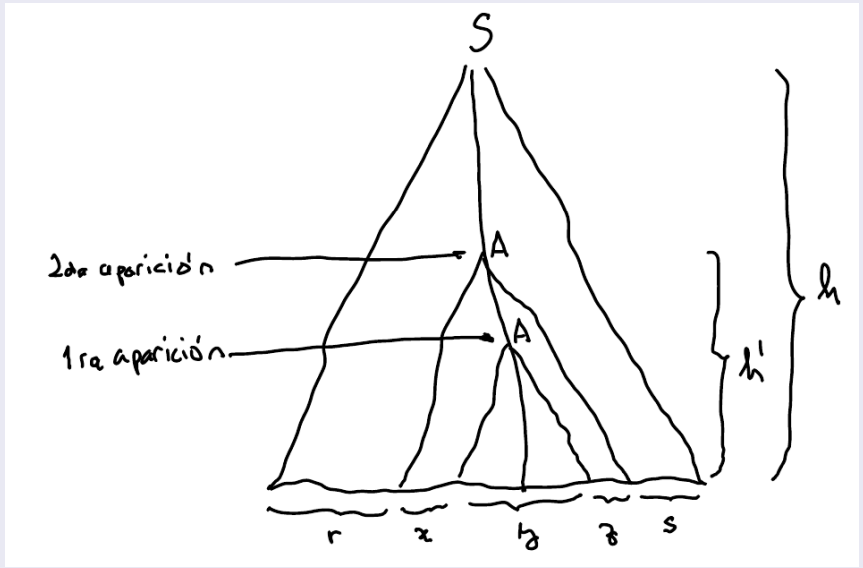
\includegraphics[scale=0.3]{imagenes/gic.pumping.tree.png}
          \end{center}
        \end{figure}

        Entonces podemos escribir \(\alpha=rxyzs\) con \(r,x,y,z\) y \(s\) como se muestra en la figura.
  \item \(|xyz|\leq n = a^{|V_n| + 1}\).
        Como \(A\) es el primer no terminal que se repite, podemos asegurar que \(h' \leq |V_N| + 1\). La segunda aparición de \(A\) tiene que pasar a lo sumo \(|V_n|\) pasos mas adelantes, sino se debería repetir otro no terminal antes. Entonces por el lema \ref{lem:altura}, resulta que \(|xyz|\leq a^{h'}\leq a^{|V_N|+1}\).
  \item \(|xz| > 0\).

        Supongamos que \(|xz| = 0\), esto quiere decir que podriamos remplazar el subárbol con raíz en la segunda aparición de \(A\) por el subárbol con raíz en la primera aparición.

        \begin{figure}[H]
          \begin{center}
            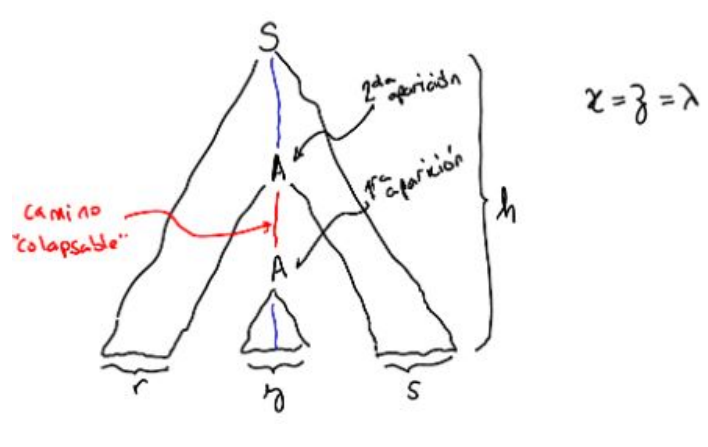
\includegraphics[scale=0.4]{imagenes/gic.pumping.tree.colapsable.png}
          \end{center}
        \end{figure}

        Esto es absurdo ya que habíamos dicho que el árbol era mínimo por lo que no debería poder colapsarse ninguno de sus caminos.

  \item \(\forall i\geq 0, rx^iyz^is\in L\)
        Finalmente, vamos a demostrar esto por inducción:
        \begin{itemize}
          \item \textbf{Caso base (\(i = 0\)):} Sabemos que \(S\deriva rAs\) y \(A\deriva y\), entonces \(S\deriva rAs\deriva rys\). Además \(rys = rx^0yz^0s\).
          \item \textbf{Paso inductivo \( i-1 \Rightarrow i\):}
                \begin{itemize}
                  \item[] \textbf{Hipotesis inductiva:} \(S\deriva rx^{i-1}Az^{i-1}s\).
                \end{itemize}
                Sabemos \(A\deriva xyz\), entonces:
                \[ S \deriva  rx^{i-1}Az^{i-1}s \Rightarrow rx^{i-1}xyzz^{i-1}s \Rightarrow rx^iyz^is \]
                Y por lo tanto \(rx^iyz^is\in L\).
        \end{itemize}
\end{enumerate}

\subsection{Propiedades de los Lenguajes Independientes del Contexto}
\begin{itemize}
  \item Si \(L_1\) y \(L_2\) son lenguajes independientes del contexto, entonces \(L_1 \cup L_2\) también lo es.
        \begin{demo}[0.8\textwidth]
          Como \(L_1\) y \(L_2\) son dos lenguajes independientes del contexto, entonces existen dos grámatica independientes del contexto \(G_1=\langle V_N, \Sigma, P_1, S_1 \rangle\) y \(G_2=\langle V_N, \Sigma, P_2, S_2 \rangle\). tales que \(L_1 = \mathcal{L}(G_1)\) y \(L_2 = \mathcal{L}(G_2)\). Supongamos, además, sin perdida de generlidad que \(V_{N_1}\cap V_{N_2} = \emptyset\). Definamos entonces:
          \[ G = \langle V_{N_1} \cup V_{N_2} \cup \{S\}, \Sigma, P_1 \cup P_2 \cup \{ S \to S_1,~S\to S_2\}, S \rangle \]

          Veamos que \(\forall\alpha\in\Sigma^*, \alpha\in\mathcal{L}(G) \iff \alpha\in\mathcal{L}(G_1) \cup \mathcal{L}(G_2)\).

          \begin{align*}
            \alpha\in\mathcal{L}(G) & \iff S\deriva\alpha \iff \red{S_1 \deriva \alpha} \lor \blue{S_2\deriva \alpha} \\
                                    & \iff \red{\alpha\in\mathcal{L}(G_1)} \lor \blue{\alpha\in\mathcal{L}(G_2)}      \\
                                    & \iff \alpha\in\mathcal{L}(G_1) \cup \mathcal{L}(G_2)
          \end{align*}
        \end{demo}
  \item Si \(L_1\) y \(L_2\) son lenguajes independientes del contexto, entonces \(L_1L_2\) también lo es.
        \begin{demo}[0.8\textwidth]
          Como \(L_1\) y \(L_2\) son dos lenguajes independientes del contexto, entonces existen dos gramáticas independientes de contexto \(G_1=\langle V_{N_1}, \Sigma, P_1, S_1 \rangle\) y \(G_2=\langle V_{N_2}, \Sigma, P_2, S_2 \rangle\) tales que \(L_1 = \mathcal{L}(G_1)\) y \(L_2 = \mathcal{L}(G_2)\). Supongamos, además, sin perdida de generlidad que \(V_{N_1}\cap V_{N_2} = \emptyset\). Definamos entonces:
        \end{demo}
        \begin{demoPart}[0.8\textwidth]
          \[ G = \langle V_{N_1} \cup V_{N_2} \cup \{S\}, \Sigma, P_1 \cup P_2 \cup \{ S \to S_1S_2\}, S \rangle \]

          Veamos que \(\forall\alpha\in\Sigma^*, \alpha\in\mathcal{L}(G) \iff \alpha\in\mathcal{L}(G_1)\mathcal{L}(G_2)\).

          \begin{align*}
            \alpha\in\mathcal{L}(G) & \iff S\deriva\alpha \iff S_1S_2\deriva\alpha                                                                            \\
                                    & \iff\exists\beta_1,\beta_2\in\Sigma^*:~\alpha=\beta_1\beta_2\land \red{S_1\deriva\beta_1}\land \blue{S_2\deriva\beta_2} \\
                                    & \iff\red{\beta_1\in\mathcal{L}(G_1)} \land \blue{\beta_2\in\mathcal{L}(G_2)}                                            \\
                                    & \iff \beta_1\beta_2 = \alpha\in\mathcal{L}(G_1)\mathcal{L}(G_2)                                                         \\
          \end{align*}
        \end{demoPart}
  \item Si \(L\) es un lenguaje independiente del contexto, entonces \(L^+\) también lo es.
        \begin{demo}[0.8\textwidth]
          Como \(L\) es un lenguaje independiente del contexto, entonces existe una gramática independiente del contexto \(G=\langle V_N, \Sigma, P, S \rangle\) tal que \(L = \mathcal{L}(G)\). Definamos entonces:

          \[ G^+ = \langle V_N \cup \{S\}, \Sigma, P \cup \{ S' \to SS',~S'\to S\}, S'\rangle \]

          Veamos que \(\mathcal{L}(G') = L^+ \)

          \begin{align*}
            \alpha\in\mathcal{L}(G') & \iff S'\deriva\alpha \iff \red{SS' \deriva \alpha}\lor\blue{S\deriva\alpha}
          \end{align*}

          Supongamos que \(\blue{S\deriva\alpha}\), entonces trivialmente vale \(\alpha\in L\subseteq L^+\).

          Por inducción, Supongamos que \(S' \deriva\beta\in L^+\): Sea \(\alpha =\gamma\beta\) con \(\gamma\in\Sigma^*\). Entonces \(SS'\deriva\alpha \iff SS'\deriva\gamma\beta \iff S\deriva\gamma \land S'\deriva\beta\)
          Entonces pasa que \(\gamma\in L\) y, por hipotesis inducción,\(\beta\in L^+\), Luego \(\gamma\beta\in L^+\)
        \end{demo}
  \item  Si \(L\) es un lenguaje independiente del contexto, entonces \(L^*\) también lo es.
        \begin{demo}[0.8\textwidth]
          Como \(L\) es un lenguaje independiente del contexto, entonces existe una gramática independiente del contexto \(G=\langle V_N, \Sigma, P, S \rangle\) tal que \(L = \mathcal{L}(G)\). Definamos entonces:
          \[
            G^* = \langle V_N \cup \{S\}, \Sigma, P \cup \{ S' \to SS',~S'\to \varepsilon\}, S'\rangle
          \]

          Veamos que \(\mathcal{L}(G^*) = L^*\). Esta demonstración es símilar a la anterior. La única defirencia es que en algún momento, en vez de usarse la regla \(S'\to S\), se usa la regla \(S'\to \varepsilon\).
        \end{demo}
  \item Si \(L_1\) y \(L_2\) son lenguajes independientes del contexto, entonces \(L_1\cap L_2\) no siempre es lenguaje independiente del contexto.
        \begin{demo}[0.8\textwidth]
          Sean \(L_1 = \{ a^n b^m c^l: n,m,l \geq 0 \land n = m \}\) y \(L_2 = \{ a^n b^m c^l : n \geq 0 \land m = l \}\) dos lenguajes independientes de contexto (\red{Demostrar?}).
          Pero \(L_1\cap L_2 = \{ a^n b^m c^l : n,m,l \geq 0 \land n = m = l \}\) no es lenguaje independiente como puede demostrarse utilizando el lema de pumping.
        \end{demo}
  \item El lenguaje \(L = \{ ww : w \in \Sigma^* \}\) no es independiente del contexto.
        \begin{demo}[0.8\textwidth]
          Sea \(L_1 = \{ a^n b^m a^n b^m:~ n,m\geq 0\}\) es tal que \(L_1 = L \cap a^* b^* a^* b^*\)
          donde \(a^* b^* a^* b^*\) es un lenguaje regular.

          La interesección entre un lenguaje regular y un lenguaje independiente de contexto da como resultado  un lenguaje independiente de contexto (\red{Demostrar?}).

          Entonces, si \(L\) fuera independiente del contexto, \(L_1\) tambien debiera serlo. Veamos que \(L_1\) no es independiente de contexto:

          Analizemos las componsiciones disponibleas para la cadena \(a^n b^n a^n b^n \in L_1\):
          \begin{figure}[H]
            \begin{center}
              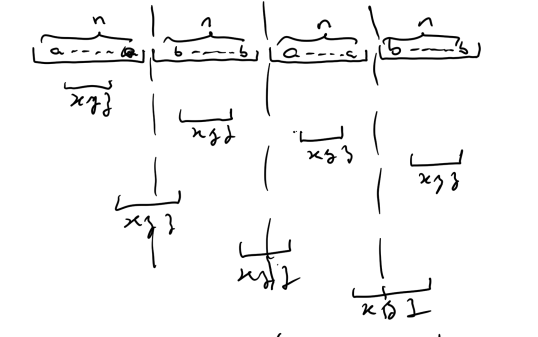
\includegraphics[scale=0.3]{imagenes/anbnanbn.png}
            \end{center}
          \end{figure}
          En los primeros cuatro casos se desbalancean la cantidad de \(a\) o \(b\), respectivamente y en el último caso se desbalancean la cantidad de \(a\) y \(b\) simultaneamente.
        \end{demo}
\end{itemize}

\subsubsection{Lenguajes libres de contexto deterministicos}
Un lenguaje \(L\) es libre de contexto deterministicos si existe un autómata de pila determinista \(A\) tal que \(L = \mathcal{L}(A)\).

Para ver más sobre lenguajes libres de contexto deterministicos, ver \href{https://www.cubawiki.com.ar/images/f/ff/TLeng_Resumen_Final_2022.pdf}{Wikipedia}.
\begin{lemma}
  El conjunto de lenguajes libres de contexto deterministicos es cerrado por la complementación.
\end{lemma}

\begin{teorema}
  Para todo automáta de pila \(M\), existe otro automáta de pila \(M'\) equivalente que siempre consume toda la cadena de entrada.
\end{teorema}
\begin{teorema}
  El complemento de un lenguaje independiente del contexto deterministico es un lenguaje independiente del contexto deterministico.
\end{teorema}
\begin{teorema}
  Existe un lenguaje independiente del contexto que es \textbf{no-deterministíco}
\end{teorema}
\begin{demo}[0.8\textwidth]
  Consideremos el lenguaje \(L = a^k b^k c^k, k\geq 0\). Sabemos que \(L\) no es independiente del contexto. Su complemento puede escribirse como:
  \begin{align*}
    \bar{L}= \{ a^i b^j c^k : i,j,k \geq 0 \land i \neq j \} \cup \{ a^i b^j c^k : i,j,k \geq 0 \land j \neq k \} \cup \overline{a^* b^* c^*}
  \end{align*}

  Osea que \(\overline{L}\) puede escribirse como la unión de dos lenguajes independientes del contexto y un lenguaje regular. Es, por lo tanto, independiente del contexto.

  Supongamosq que \(\overline{L}\) es un lenguaje independiente del contexto deterministico. Entonces, \(\overline{\overline{L}}\) también debería serlo por el teorema anterior. Pero \(\overline{\overline{L}} = L\) que ni siquiera es un lenguaje independiente del contexto. Luego \(\overline{L}\) no es deterministico.
\end{demo}

\subsection{Gramáticas propias}
\subsubsection{Conjunto de símbolos activos}
\paragraph{Símbolo alcanzable:} Dada una grámatica \(G=\langle V_N, V_T, P, S\rangle\), un símbolo \(A\in V_N\) es alcanzable si existe una forma sentencial que lo contiene,  \(S\deriva \dots A\dots\).

\paragraph{Símbolo activo:} Dada una grámatica \(G =\langle V_N, V_T, P, S\rangle\) un símbolo \(A\in V_N\) es activo si existe \(\alpha\in V_T^*\) tal que \(A\deriva \alpha\).

\paragraph{Símbolo útil:} Un no terminal \(A\) es útil si y solo si es parte de una forma sentencial que genera una cadena de terminales, osea, si \(S\deriva \alpha A\beta \deriva \omega\) con \(\omega \in \Sigma^*\) y \(\alpha, \beta \in (V_T\cup V_N)^*\).

\paragraph{Algoritmos para conseguir el conjunto de no-terminales activos de una gramática:}
\begin{algorithmic}
  \Function{activos}{\(\langle V_N, V_T, P, S\rangle\): Gramática}
  \State \(\texttt{Act}\gets\emptyset\)
  \Repeat
  \For{\(A\to \alpha \in P\)}
  \If{\(\alpha \in (\texttt{A}\cup V_T)^*\)}
  \State\(\texttt{Act}\leftarrow\texttt{Act}\cup \{A\}\)
  \EndIf
  \EndFor
  \Until{ \texttt{Act} no cambie}
  \State \Return \texttt{Act}
  \EndFunction
\end{algorithmic}

\subsubsection{Conjunto de símbolos anulables}
\begin{lemma}
  Sea G una gramática libre de contexto. Entonces existe una grámatica propia (sin producciones borradoras) \(G'\) tal que genere el mismo lenguaje que G sin la cadena nula.
\end{lemma}

\paragraph{No terminal anulable:} Un no terminal \(A\) es anulable si y solo  \(A\deriva \varepsilon\).

\paragraph{Algoritmo para conseguir el conjunto de no terminales anulables de una gramática:}

\begin{algorithmic}
  \Function{anulables}{\(\langle V_N, V_T, P, S\rangle\): Gramática}
  \State \(\texttt{An}\gets\emptyset\)
  \For{\(A\to \alpha \in P\)}
  \If{\(\alpha = \lambda\)}
  \State\(\texttt{An}\leftarrow\texttt{An}\cup \{A\}\)
  \EndIf
  \EndFor
  \Repeat
  \For{\(A\to \alpha \in P\)}
  \If{\(\alpha \in \texttt{An}^*\)}
  \State\(\texttt{An}\leftarrow\texttt{An}\cup \{A\}\)
  \EndIf
  \EndFor
  \Until{ \texttt{An} no cambie}
  \State \Return \texttt{Anul}
  \EndFunction
\end{algorithmic}

\subsubsection{Gramáticas reducidas}
\paragraph{Grámatica reducida:} Una gramática \(G = \langle V_N, V_T, P, S\rangle\) es reducida si y solo si para todo \(A\in V_N\) se cumple que \(A\) es alcanzable y activo.
\paragraph{Algoritmo para conseguir una gramática propia:}

\begin{algorithmic}
  \Function{propia}{\(G=\langle V_N, V_T, P, S\rangle\): Gramática}
  \State \(\texttt{An}\gets\texttt{anulables}(G)\)
  \For{\(A\to \alpha \in P\)}
  \If{\(\alpha = X_1\dots X_k\) con \(X_{j_1}, \dots, X_{j_m} \in \texttt{An}\)}
  \State Agregar todas las producciones \(A\to\alpha'\) donde las \(\alpha'\) se obtiene eliminando cada subconjunto en \(X_{j_1}, \dots, X_{j_m}\) de \(\alpha\). Si todos los símbolos de \(\alpha\) son anulables, no agregar \(A\to \lambda\).
  \EndIf
  \If{\(\alpha = \lambda\)}
  \State Eliminar la producción \(A\to \lambda\)
  \EndIf
  \EndFor
  \State \Return G modificada
  \EndFunction
\end{algorithmic}

\subsubsection{Forma normal de Chomsky}
Una gramática \(G = \langle V_N, V_T, P, S\rangle\) está en forma normal de Chomsky si y solo si todas sus producciones son de la forma \(A\to BC\) o \(A\to a\), donde \(A, B, C \in V_N\) y \(a \in V_T\).

Si \(L\) un lenguaje independiente del contexto tal que \(\lambda\notin L\) entonces existe una gramática \(G\) en forma normal de Chomsky.

\subsubsection{Forma normal de Greibach}
Una gramática \(G = \langle V_N, V_T, P, S\rangle\) está en forma normal de Greibach si y solo si todas sus producciones son de la forma \(A\to a\alpha\) donde \(A\in V_N\), \(a\in V_T\) y \(\alpha \in V_N^*\).

Si \(L\) un lenguaje independiente del contexto tal que \(\lambda\notin L\) entonces existe una gramática \(G\) en forma normal de Greibach.

\subsection{Otras propiedades}
\begin{itemize}
  \item Si \(M = \langle Q, \Sigma, \delta, q_0, Z_0, F\rangle\) es un autómata de pila y \(L\) el lenguaje tal que \(L = \mathcal{L}_\lambda(M)\), entonces \(L\) es independiente del contexto.
  \item Sea \(G = \langle V_N, V_T, P, S\rangle\) una grámatica independiente del contexto. Se puede construir un autómata de pila  M tal que \(\mathcal{L}(G) = \mathcal{L}_\lambda(M)\).
\end{itemize}

\newpage
\section{Máquinas de Turing}
El modelo más básico de una máquina de turing  consiste en un control finito, una cinta infinita dividida en celdas y una cabeza de lectura. Cada celda de la cinta puede contener un único símbolo del alfabeto finito de la cinta.

Inicialmente, la cinta contiene una cadena de símbolos de entrada, seguida de un símbolo especial llamado blanco. La cabeza de lectura se coloca sobre el primer símbolo de la cadena de entrada. La máquina de Turing puede leer y escribir símbolos en la cinta o mover la cabeza de lectura a la izquierda o a la derecha.
\begin{figure}[H]
  \begin{center}
    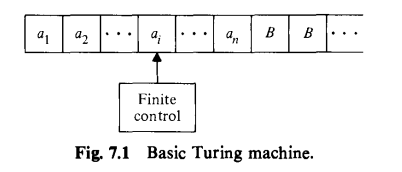
\includegraphics[scale=0.75]{imagenes/mt.png}
  \end{center}
\end{figure}
Formalmente, definimos la máquina de Turing (MT) \(M\) como una tupla:
\[
  M = \langle Q, \Sigma, \Gamma, \delta, q_0, B, F \rangle
\]

Donde:
\begin{itemize}
  \item \(Q\) es un conjunto finito de estados.
  \item \(\Sigma\) es un alfabeto de entrada.
  \item \(\Gamma\) es un alfabeto de cinta.
  \item \(\delta: Q\times\Gamma\to Q\times\Gamma\times\{L, R\}\) es una función de transición. Podría estar indefinido para algunos argumentos. La función indica devuele el estado al que se debe pasar, el símbolo a escribir en la posición actual de la cinta y el movimiento del cabezal (izquierda o derecha).
  \item \(q_0 \in Q\) es el estado inicial.
  \item \(B \in \Gamma\) es el símbolo blanco.
  \item \(F \subseteq Q\) es el conjunto de estados finales.
\end{itemize}

\paragraph{Configuración instantanea:} Una configuración instantánea de una MT es una tupla \(\alpha_1 q \alpha_2\) donde \(q\in Q\) y \(\alpha_1,\alpha_2\in\Gamma^*\) donde:
\begin{itemize}
  \item \(\alpha_1\) son los simbolos de la cinta a la izquierda del cabezal.
  \item \(q\) es el estado actual.
  \item \(\alpha_2\) son los símbolos de la cinta a la derecha del cabezal hasta el último símbolo distinto de \(B\).
\end{itemize}
Notemos que \(\alpha_1,\alpha_2\in\Gamma^*\), osea que pueden tener apariciones de \(B\).

Asumismos que el cabezal está escaneando el símbolo más a la derecha de \(\alpha_2\) o un blanco si \(\alpha_2=\lambda\).

\paragraph{Movimiento del cabezal:} El movimiento del cabezal se define como sigue: Sea \[X_1\dots X_{i-2}qX_{i}\dots X_n\]una configuración instantánea de una MT \(M\).

Supongamos que \(\delta(q,X_i) = (p, Y, L)\):
\begin{itemize}
  \item Si \(i -1 = n\), asumimos \(X_i = B\)
  \item Si \(i = 1\) entonces es imposible moverse a la izquierda.
  \item Si \(1 < i < n\) entonces escribimos:
        \[
          X_1\dots X_{i-1}qX_{i}\dots X_n \underset{M}{\vdash} X_1\dots X_{i-2}pX_{i-1}YX_{i+1}\dots X_n
        \]

        En caso de haya algún sufijo de \(X_{i-1}YX_{i+1}\dots X_n\) que sea completamente blanco, entonces se elimina.
\end{itemize}

Similarmente, si \(\delta(q,X_i) = (p, Y, R)\):
\[
  X_1\dots X_{i-1}qX_{i}\dots X_n \underset{M}{\vdash} X_1\dots X_{i-1}YpX_{i+1}\dots X_n
\]

Si dos configuraciónes instantáneas están relacionadas por \(\resulta{M}\), entonces decimos que la segunda es un resultado de la primera.

Si una configuración instantánea resulta de otra en un número fínito de pasos, entonces están relacionadas por el símbolo \(\resultam{M}\).

\paragraph{Lenguaje aceptado por una MT:} Definimos al lenguaje aceptado por una MT \(M=\langle Q, \Sigma, \Gamma, \delta, q_0, B, F \rangle\) como:
\[
  \mathcal{L}(M) = \{ \omega \in \Sigma^*  : q_0\omega \resultam{M} \alpha_1 p\alpha_2 \text{ con } p\in F \land \alpha_1,\alpha_2\in\Gamma^* \}
\]

Asumimos que la máquina de Turing se detiene cuando el input es aceptado. Además es posible que nunca se detenga si el input no es aceptado.

\subsection{Autómatas linealmente acotados}
Es una máquina de Turing  no deterministica que cumple con las siguientes condiciones:
\begin{enumerate}
  \item El alfabeto de entrada incluye dos símbolos especiales (\textcentoldstyle~y \textdollar) que son utilizados como topes izquierdo y derecho, respectivamente.
  \item El autómata no se mueve ni a la izquierda de \textcentoldstyle ni a la derecha de \textdollar, ni los sobreescribe.
\end{enumerate}

\subsubsection*{Máquinas de dos cintas}
Una máquina de Turing con dos o más cintas puede simularse usando la defición dada anteriormente. Para ello, definimos los estados en \(\Gamma\) como tuplas \([x_1, x_2]\) donde \(x_i\) sería el símbolo guardado en la \(i\)-ésima cinta.


\begin{teorema}
  Si \(L\) es un lenguaje dependiente del contexto, entonces existe un autómata linealmente acotado \(A\) tal que \(\mathcal{L}(A) = L\).
\end{teorema}

\begin{demo}[0.8\textwidth]
  Se construye el autómata linealmente acotado \(M\) tal que:
  \begin{enumerate}
    \item La primera cinta contiene la cadena de entrada \textcentoldstyle\(\omega\)\textdollar.
    \item La segunda cinta se utiliza para generar las formas de la derivación. En cualquie instante, esta cinta contendrá la forma sentencial \(\alpha\) que representa la derivación de la cadena de entrada. Se inicializa con el símbolo distingido \(S\).
  \end{enumerate}

  El autómata funcionará de la siguientes manera:
  \begin{enumerate}
    \item Si \(\omega=\lambda\), entonces \(M\) se detiene rechanzando la cadena de entrada.
    \item Sino:
          \begin{enumerate}
            \item Selecciona (en forma no deterministica) la posición \(i\) dentro de \(\alpha\) (la derivación que se encuentra en la cinta)
            \item Selecciona (en forma no deterministica) la producción \(\beta\to\gamma\in P\).
            \item Si \(\beta\) aparece a partir de la posición \(i\) en \(\alpha\), entonces remplaza \(\beta\) por \(\gamma\) en \(\alpha\).
            \item Si la nueva forma sentencial \(\alpha\) es tal que \(|\alpha| > |\omega|\), entonces \(M\) se detiene rechazando la cadena de entrada.
            \item Sino, comparamos \(\alpha\) con \(\omega\). Si son iguales, entonces \(M\) se detiene aceptando la cadena de entrada. Sino, se vuelve a repetir el paso 2.
          \end{enumerate}
  \end{enumerate}
\end{demo}

\subsection{Lenguajes recursivos}
Son lenguajes \(L\) sobre un alfabeto \(\Sigma\) para el cual existe una máquina de Turing que se detiene para todo \(\alpha\in\Sigma^*\) y la acepta (termina en un estado final) si \(\alpha\in L\) o la rechaza (termina en un estado no final) si \(\alpha\notin L\). En otras palabras, son los lenguajes para los cuales existe un algoritmo que permite decidir la pertenencia (o no) de toda cadena al lenguaje.

\begin{teorema}\label{teorema:recursividad}
  Todo lenguaje dependiente del contexto es recursivo
\end{teorema}

\begin{demo}[0.8\textwidth]
  Sea \(G=\langle N, \Sigma, P, S \rangle\) un gramática dependiente del contexto y \(\omega\in\Sigma^*\). Vamos a construir un grafo fínito en el cual cada nodo tiene asocida un \(\alpha\in(V_N\cup V_T)^+\) con \(|\alpha| \leq |\omega|\). Las arista representas una producción de \(G\), osea si \(\gamma_1\tau\gamma_2\) y \(\gamma_1\beta\gamma_2\) son dos nodos, entonces van a estar conectados si y solo si \(\tau\to\beta\in P\).

  Por ser \(G\) dependiente del contexto, vale \(|\tau|\leq |\beta|\), entonces \(|\gamma_1\tau\gamma_2|\leq |\gamma_1\beta\gamma_2|\). Por lo tanto, el grafo es acotado.

  En este grafo finito, es cierto que \(S\underset{G}{\deriva}\omega\) si y solo si existe un camino desde el nodo correspondiente a \(S\) hasta el nodo correspondiente a \(\omega\). Y esto último es decidible, o sea, tiene algoritmo. Por lo tanto, \(G\) es recursivo.
\end{demo}

\begin{lemma}
  Sea \(M_1, M_2, \dots\) una enumeración de un conjunto de máquinas de Turing que paran para todas las entadradas. Siempre existe un lenguaje recursivo que no es aceptado por ninguna de ellas, o sea, siempre existe un lenguaje \(L\) tal que \(L\) es recursivo y \(L\notin\mathcal{L}(M_i)\) para todo \(i\).
\end{lemma}

\begin{demo}[0.8\textwidth]
  Consideremos el lenguaje definido \( L = \{ \omega_i : \omega_i \notin \mathcal{L}(M_i)\}\), es decir \(L\) está formado por todas las cadenas que son rechazadas por alguna de las máquinas \(M_i\). Como es decidible si \(\omega_i\in L\) o no (pues simplemente corremos las \(M_i\) con entrada \(\omega\) y vemos si para en un estado no final), entonces \(L\) es recursivo.

  Supongamos ahora que este lenguaje es aceptado por alguna de las máquinas enumeradas. Sea \(M_j\), la misma. Entonces ¿que pasa si \(\omega_j\in L\)?

  Por definición de \(L\) tenemos que \(w_j\in L \iff w_j\notin \mathcal{L}(M_j) \iff w_j \notin L\). Esto es un absurdo, por lo tanto \(L\) no es aceptado por ninguna máquina \(M_1,M_2,\dots\).
\end{demo}

\begin{lemma}
  Existe un lenguaje recursivo que no es dependiente del contexto
\end{lemma}
\begin{demo}[0.8\textwidth]
  Vamos a tratar de demostrar que podemos encontrar una numeración de máquinas Turing correspondientes a cada uno de los lenguajes dependientes del contexto definidos sobre \(\{0,1\}^*\).
\end{demo}
\begin{demoPart}[0.8\textwidth]
  Estas máquinas de Turing paran en todas las entradas porque como los lenguajes son dependientes de contexto, siempre hay un algoritmo de reconomcimiento cuando el lenguaje es dependiente del contexto.

  Codifiquemos todas estas gramaticas con cadenas binarias, es decir, demos una representación binaria a cada símbolo de la gramática codificando:

  \begin{itemize}
    \item \(0 = 10\)
    \item \(1 = 100\)
    \item y al resto de los simbolos \(s_k = 10^k\)
  \end{itemize}

  Gracias a esta codificación mediante 0s y 1s, podemos enumerarlas de la siguientes manera: \(G_1,G_2,\dots\). Además, por el teorema \ref{teorema:recursividad}, existen autómatas \(M_1, M_2,\dots\) que aceptan los lenguajes generados por cada una de ellas.

  Luego, por el lema, anterior, tenemos que existe un lenguaje \(L\) recursivo que no es aceptado por ninguno de estos autómatas y no es dependiente del contexto.
\end{demoPart}
\subsection{Máquinas de Turing No Deterministicas}
\begin{teorema}
  Sea \(M\) una máquina de Turing no deterministica y \(L = \mathcal{L}(M)\). Entonces existe una máquina de Turing determinista \(M'\) que acepta el mismo lenguaje.
\end{teorema}

\begin{demo}[0.8\textwidth]
  Sea \(r\) la máxima cantidad posible de transiciones que parte de un estado cualquiera de \(M\). Numeremos, para cada estado, las transiciones que parten de él con números entre 1 y \(r\).

  Entonces toda secuencia finita de enteros entre 1 y \(r\) representa un camino en \(M\) partiendo desde el estado inicial \(q_0\). Algunas de estas secuencias no serán ejecutables por no existir alguna de sus transiciones.

  Podemos construir una máquina de turing \(M'\) de tres cintas tal que:
  \begin{itemize}
    \item La primera contiene la entrada de \(M\)
    \item La segunda, una secuencia de enteros entre 1 y \(r\) que corresponderá a una secuencia de transiciones a partir del estado inicial \(q_0\).
    \item La tercera servirá para simular la \(M\).
  \end{itemize}
  Y funcionará de la siguiente manera:
  \begin{itemize}
    \item Generamos secuencias de enteros con valroes entre 1 y \(r\) en orden creciente de longitud y alfabetico, que irán siendo escritos en la segunda cinta.
    \item Para cada secuencia:
  \end{itemize}
\end{demo}
\begin{demoPart}[0.8\textwidth]
  \begin{itemize}
    \item[]
      \begin{enumerate}
        \item Borramos el contenido de la cinta 3
        \item Copiamos el contenido de la cinta 1 en la cinta 3.
        \item Simulamos la MT en la cinta 3 ejecutando la secuencia de transiciones en la cinta 2.
        \item Aceptamos la cadena de la cinta 1 si se acepta esa cadena en la simulación que corremos en la cinta 3.
      \end{enumerate}
    \item Cuando la cadena analizada no es aceptada por \(M\), \(M'\) no parará.
  \end{itemize}
\end{demoPart}

\begin{teorema}
  Sea \(L\) el lenguaje de la gramática \(G = \langle V_N, V_T, P, S\rangle\). Entonces existe una máquina de Turing \(M\) que acepta el mismo lenguaje.
\end{teorema}

\begin{demo}[0.8\textwidth]
  Podemos construir una máquina de Turing \(M\) no deterministica de dos cintas tal que:
  \begin{itemize}
    \item la primera contiene la cadena de entrada \(\omega\)
    \item La segunda contiene la forma setencial \(\alpha\) de la derivación de la cadena de entrada. Se inicializa con el símbolo inicial de la gramática \(S\).
  \end{itemize}

  Y opera de la siguiente manera:
  \begin{enumerate}
    \item Seleccionar (en forma no-deterministica) la posición \(i\) dentro de \(\alpha\)
    \item Seleccionar de forma no-deterministica una regla de producción \(\beta \rightarrow \gamma\in P\)
    \item Si \(\beta\) aparece a partir de la posición \(i\) en \(alpha\), entonces reemplazar \(\beta\) por \(\gamma\) en \(alpha\).
    \item Comparar la nueva forma sentencial \(\alpha\) con la cadena de entrada \(\omega\). Si son iguales, entonces aceptar la cadena de entrada. Si no, volver al paso 1.
  \end{enumerate}
\end{demo}

\begin{teorema}
  Sea \(L\) el lenguaje aceptado por una máquina de Turing \(M\). Entonces existe una gramática sin restricciones \(G\) que genera el mismo lenguaje.
\end{teorema}

\begin{demo}[0.8\textwidth]
  Vamos a armar una gramática que genere dos copias de alguna representación de la cadena de entrada y que luego simule la operación de la maquina de Turing sobre una de ellas. Si esta simulación resulta en una aceptación, entonces la primera copia se convierte en la cadena igual a la de entrada.
\end{demo}
\begin{demoPart}[0.9\textwidth]
  Entonces sea \(M= \langle Q, \Sigma, \Gamma, \delta, q_0, B, F\rangle\) una máquina de Turing que acepta el lenguaje \(L\). Definimos la gramática \(G = \langle V_N, \Sigma, P, A_1  \rangle\) de la siguiente manera:
  \begin{itemize}
    \item \(V_N = ((\Sigma\cup\{\lambda\})\times\Gamma)\cup\{A_1,A_2,A_3\}\)
    \item \(P\) contiene las siguientes producciones:
          \begin{itemize}
            \item \(A_1 \rightarrow q_0A_2\)
            \item  \(A_2 \rightarrow [a,a]A_2\) para cada \(a\in\Sigma\)
            \item \(A_2\to A_3\)
            \item \(A_3\to [\lambda, B]A_3\)
            \item \(A_3\to \lambda\)
            \item \(q[a,X]\to [a, Y]p\) para cada \(q\in Q, a\in\Sigma\cup\{\lambda\}, X,Y\in\Gamma\) tales que \(\delta(q,X) = (p,Y, R)\)
            \item \([b, Z]q[a,X]\to p[b,Z][a, Y]\) para todo \(q\in Q, a,b\in\Sigma\cup\{\lambda\}, X,Y,Z\in\Gamma\) tales que \(\delta(q,X) = (p,Y, L)\)
            \item \([a,X]q\to qaq\), \(q[a,X]\to qaq\), \(q\to\lambda\) para todo \(q\in F, a\in\Sigma\cup\{\lambda\}, X\in\Gamma\)
          \end{itemize}
  \end{itemize}
  Utilizando las reglas 1 y 2 se puede generar \(A_1 \deriva q_0[a_1,a_1]\dots[a_n,a_n]A_2\)

  Luego, con la regla 3 se generan los símbolos correspondientes a los a los espacios en blancos necesarios para el analísis de la cadena de entrada en \(M\):
  \[ A_1 \deriva q_0[a_1,a_1]\dots[a_n,a_n][\lambda, B]^mA_3\]

  Utilizando las reglas 6 y 7 se simula la operación de la máquina de Turing sobre las segundas componentes, dejando intactas las primeras componentes.

  Veamos que:

  \[ q_0a_1\dots a_1\resultam{M} X_1\dots X_{r-1}qX_r\dots X_s\Rightarrow \]
  \[q_0[a_1,a_1]\dots[a_n,a_n][\lambda, B]\underset{G}{\deriva} [a_1,X_1]\dots[a_{r-1,X_{r-1}}]q[a_r,X_r]\dots[a_{n+m},X_{n+m}]\]
  con \(a_1,\dots,a_n\in\Sigma\), \(X_1,\dots,X_{n+m}\in\Gamma\), \(a_{n+1} = \dots = a_{n+m} = \lambda\), \(X_{n+1} = \dots = X_{n+m} = B\).


  Para \(\overset{0}{\vdash}\) vale trivialmente pues:
  \begin{itemize}
    \item \(q_0a_1\dots a_n\overset{0}{\vdash} q_0a_1\dots a_n\)
    \item y \(q_0[a_1,a_1]\dots[a_n,a_n][\lambda, B]^m\overset{0}{\Rightarrow} q_0[a_1,a_1]\dots[a_n,a_n][\lambda, B]^m \)
  \end{itemize}

  Ahora, probemos por introduccion que vale lo mismo para \(\overset{k}{\vdash}\) si vale para \(\overset{k-1}{\vdash}\). Supongamos que \(q_0a_1\dots a_n\overset{k}{\vdash} q_0a_1\dots a_n\). Entonces:
\end{demoPart}
\begin{demoPart}[0.8\textwidth]
  Suponiendo que vale
  \[ q_0a_1\dots a_1\overset{k-1}{\resulta{M}} X_1\dots X_{r-1}qX_r\dots X_s\Rightarrow \]
  \[q_0[a_1,a_1]\dots[a_n,a_n][\lambda, B]\underset{G}{\deriva} [a_1,X_1]\dots[a_{r-1,X_{r-1}}]q[a_r,X_r]\dots[a_{n+m},X_{n+m}]\]

  Si en el paso \(k\), el movimiento es hacia la derecha, o sea \(\delta(q,X_r) = (p, Y_r, R)\), por la regla 6 sabemos que \(q[a_r,X_r]\to[a_r, Y_r]p\in P\), por lo que

  \[[a_1,X_1]\dots[a_{r-1,X_{r-1}}]q[a_r,X_r]\dots[a_{n+m},X_{n+m}]\deriva\]
  \[ [a_1,X_1]\dots[a_{r},Y_{r}]p[a_{r+1},X_{r+1}]\dots[a_{n+m},X_{n+m}]\]

  Si en el paso \(k\), el movimiento es hacia la izquierda, o sea \(\delta(q,X_r) = (p, Y_r, L)\) entonces por la regla 7 sabemos que \([a_{r-1}, X_{r-1}]q[a_r,X_r]\to p[a_{r-1}, X_{r-1}][a_r, Y_r]\in P\) por lo que:

  \[[a_1,X_1]\dots[a_{r-1,X_{r-1}}]q[a_r,X_r]\dots[a_{n+m},X_{n+m}]\deriva\]
  \[ [a_1,X_1]\dots p[a_{r-1},Y_{r-1}][a_{r},X_{r}]\dots[a_{n+m},X_{n+m}]\]

  Entonces, si llegamos a una forma sentencial en la que el estado \(q\) sea final, aplicando repetidas veces la regla 8 tenemos que queda cualquiera de las dos derivaciones va a derivar en algo del estilo \(a_1 a_2\dots a_n\).

  En el sentido inverso, tambien puede \red{demostrarse} que si \(\alpha\in\mathcal{L}(G)\) entonces \(x\in\mathcal{L}(M)\)
\end{demoPart}

\subsection{Lenguajes recursivamente enumerables}
Los lenguajes recursivamente enumerables son lenguajes para los que existe una máquina de turing que puede enumerar todas las cadenas válidas del mismo. Si el lenguaje es infinito, entonces se puede elegir un algoritmo que evite repeticiones.

Los lenguajes regulares, los libres de contexto, los dependientes del contexto y los recursivos son lenguajes recursivamente enumerables.

\subsubsection*{Codificación de máquinas de Turing restringidas a u alfabeto binario}

Sea \(M = \langle Q, \{0,1\}, \{0,1,B\}, \delta, q_1, B,\{q_2\}\rangle\) una máquina de Turing con \(Q = \{q_1, q_2,\dots,q_n\}\) el conjunto de estados. Entonce, si usamos \(X_1 = 0\), \(X_2 = 1\), \(X_3 = B\), \(D_1 = L\) y \(D_2 = R\). Entonces podemos codificar cada transición \(\delta(q_i, X_j) = (q_k, X_l, D_m)\) como una cadena de la forma \(0^i10^j10^k10^l10^m 1\). Y el código binario para la máquina de Turing \(M\) es la concatenación de todas las cadenas de transiciones de la siguiente forma: \(111trans_111\dots11trans_r111\).

\begin{teorema}
  Existe un lenguaje que no es recursivamente enumerable.
\end{teorema}
\begin{demo}[0.8\textwidth]
  Ordenemos el conjunto \(\{0,1\}^*\) primero por longitud y luego siguiendo el orden léxico. Llamemos \(w_i\) a la \(i-\)ésima cadnea según este ordenamientos y \(M_j\) a la máquina de Turing cuyo código binario es el entero positivo \(j\).

  Entonces podemos construir una tabla que indique con un 1 en la entrada \(i,j\) si \(w_i\in\mathcal{M_j}\) y un 0 cuando no.

  Definamos el lenguaje \(L_d\) como \[ L_d = \{w_i \mid w_i\notin \mathcal{L}(M_i)\}\] que corresponde a los ceros de la diagonal de la tabla.

  Si \(L_d\) es recursivamente enumerable, entonces existe una máquina de Turing \(M_j\) tal que \(\mathcal{L}(M_j) = L_d\). Pero entonces, \(w_j\notin L_d \iff w_i \notin \mathcal{L}(M_i) \iff w_j\notin L_d\) lo que es una contradicción.

  Luego \(L_d\) no es recursivamente enumerable.
\end{demo}

\paragraph{Lenguaje universal:} Definimos \(L_u\) como el lenguaje constituido por todos los pares de máquinas de Turing \(M\)- cadena de entrada \(\omega\) tales que \(\omega\in\mathcal{L}(M)\):

\[ L_u = \{ (M, \omega) \mid \omega\in\mathcal{L}(M)\}\]

\begin{teorema}
  \(L_u\) es recursivamente enumerable.
\end{teorema}

\begin{demo}[0.8\textwidth]
  Para demostrarlo vamos a crear una máquina de Turing de 3 cintas que acepta \(L_u\) de la siguiente manera:
  \begin{itemize}
    \item La cinta 1 contiene la cadena de entrada, o sea, la codificación de la máquina \(M\) seguida de la cadena\(\omega\).
    \item La segunda cinta se utiliza para simular la cinta de la máquina de turing original.
    \item La tercera cinta contiene el estado actual de la máquina de turing simulada.
  \end{itemize}
  La máquina funciona de la siguiente mánera:
  \begin{enumerate}
    \item Chequear que la cadena que codifica la máquina turing de \(M\) en la cinta 1 sea sintácticamente correcta y determinística.
    \item Inicilizar la cinta 2 con la cadena de entrada y la cinta 3 con 0 (que representa el estado inicial \(q_1\)). Todas las cabezas deben posicionarse en la posición extrema izquierda de sus respectivas cintas.
  \end{enumerate}
\end{demo}
\begin{demoPart}[0.8\textwidth]
  \begin{enumerate}[3.]
    \item Simular la máquina de turing
          \begin{enumerate}
            \item Si el contenido de la cinta 3 es 00 (correspondiente al estado \(q_2\)), entonces terminar y aceptar.\label{paso:aceptar}
            \item Sea \(X_j\) es el símbolo actualmente leído en la cinta 2 y sea \(0^i\) el contenido de la cinta 3 (estado actual \(q_i\)), entonces:
                  \begin{enumerate}
                    \item Comenzando desde la posición extrema izquierda, buscar en la cinta 1 la cadena \(110^i10^j1\) (correspondiente a \(d(q_i, X_j)\)) hasta encontrarla o hasta encontrar la cadena 111.
                    \item Si se encontró la cadena 111 entonces parar y rechazar
                    \item Si se encontró la cadena \(110^i10^j1\) entonces esto indicará que la transición que se debe realizar es \(d(q_i, X_j) = (q_k, X_l, D_m)\), osea \(0^i10^j10^k10^l10^m\). Entonces poner en la cinta 3 \(0^k\) y en la cinta 2 \(X_l\) en la posición actual y moverse en la dirección \(D_m\).
                    \item Volver al paso \ref{paso:aceptar}
                  \end{enumerate}
          \end{enumerate}
  \end{enumerate}
\end{demoPart}

\begin{teorema}
  El lenguaje \(L_u\) no es recursivo
\end{teorema}

\begin{demo}[0.8\textwidth]
  Supongamos que existe un algoritmo para reconocer \(L_u\) entonces podriamos construir un algoritmo para reconocer su complemento que es el leguaje \(L_d\).

  Pero entonces \(L_d\) sería recursivamente enumerable. Absurdo
\end{demo}

\newpage
\chapter{La que da Vero}
\section{Transformación de gramáticas}
Dada una expresión en un lenguaje formal, buscamos encontrar un algoritmo que permita, a la computadora, entenderla. Para esto debemos realizar los siguientes pasos:
\begin{enumerate}
  \item Revisar que la expresión solamente tenga símbolos del alfabeto del lenguaje.
  \item Revisar que la expresión tenga una forma que respete la grámatica.
  \item Mapear la expresión, usando la grámatica, a una estructura de datos que pueda ser procesada por la computadora.
\end{enumerate}

Los lenguajes que no son recursivamente enumerables no pueden ser reconocidos por ninguna máquina de Turing.

Los lenguajes regulares y algunos lenguajes libres de contexto se pueden analizar en tiempo lineal con respecto al tamaño de la entrada.

El analísis de los demás lenguajes libres de contexto se puede realizar en tiempo polinomial con respecto al tamaño de la entrada. Y para lenguajes arbirtrarios no hay cota en la comlejidad computaciónal para analizarlos.

\subsection{Definiciones para recordar}
\paragraph{Alfabeto:} Conjunto finito de símbolos.
\paragraph{Cadena:} Secuencia finita de símbolos de un alfabeto.
\paragraph{Lenguaje:} Conjunto de cadenas.

Hay lenguajes naturales y lenguajes formales. Los segundos se definen matemáticamente mediante grámaticas y/o autómatas.

\paragraph{Grámatica:} Una grámatica formal es una cuádrupla \(G = (N, T, S, P)\) donde:
\begin{itemize}
  \item[] \(N\) es un conjunto finito de símbolos no terminales (Variables).
  \item[]  \(T\) es un conjunto finito de símbolos terminales (Constantes).
  \item[]  \(S\) es un símbolo distinguido de \(N\)no terminal que representa el símbolo inicial.
  \item[]  \(P\) es un conjunto finito de reglas de producción de la forma \(A \rightarrow \alpha\), donde \(A,\alpha \in (N\cup T)^*\).
\end{itemize}

\paragraph{Derivación:} Sea \(G = (N, T, S, P)\) una grámatica formal. Si \(\alpha,\beta,\gamma_1,\gamma_2 \in (N\cup T)^*\) y \(\alpha \in \beta\), entonces \[\gamma_1\alpha\gamma_2\rightarrow \beta\].

La relación \(\Rightarrow\) es el subconjunto \(N\cup T)^*\times (N\cup T)^*\) y significa derivar en un solo paso.

Las relacioens \(\overset{+}{\Rightarrow}\) y \(\overset{*}{\Rightarrow}\) son la clausura transitiva y reflexo-transitiva de \(\Rightarrow\), respectivamente.

El lenguaje generado por la grámatica \(G\) es: \[ \mathcal{L}(G) = \{ \alpha\in V_T^*:~S\overset{+}{\underset{G}{\implies}}\alpha\}\]

\subsubsection{Jerarquía de Chomsky}
Es una clasifición jerarquica de tipos de grámaticas formales que generan lenguajes formales:

\begin{itemize}
  \item \textbf{Tipo 0}: Gramáticas sin restricciones. Son todos los lenguajes aceptados por una máquina de Turing y se los llama lenguajes recursivamente enumerables.
  \item \textbf{Tipo 1}: Gramáticas sensibles al contexto. Las reglas son de la forma \(\alpha\to\beta\) con \(|\alpha|<|\beta|\) y \(\alpha,\beta\in(N\cup T)^*\).

        Son aceptados por autómatas linealmente acotados que son máquinas de Turing determínisticas cuya cinta  de memoria está acotada por un múltiiplo de la longitud de entrada.

        Reconocer este tipo de lenguajes es un problema PSPACE-completo.

  \item \textbf{Tipo 2:} Gramáticas libres de contexto. Las reglas son de la forma \(A\to\gamma\) con \(A\) un no terminal y \(\gamma\) una cadena de no terminales y terminales.

        Estas grámaticas generan todos los lenguajes aceptados por automátas de pila.

        No es cierto que para cada autómata de pila no deterministico exista uno deterministico equivalente.

        Los lenguajes libres de contexto aceptados por autómatas de pila deterministicos se llaman lenguajes LR y se los puede reconocer en tiempo lineal en el tamaño de la entrada.

        Un subconjunto propio de los lenguajes LR son los generados por grámaticas LL y el algoritmo para reconocerlos es muy sencillo.

        Para reconocer un lenguaje libre de contexto no determínistico hay un algoritmo de complejidad cúbica en el tamaño de la entrada.

  \item \textbf{Tipo 3:} Gramáticas regulares. Las reglas son de la forma \(A\to a\) ó \(A\to aB\) con \(A, B\) símbolos no terminales y \(a\) un símbolo terminal.

        Alternativamente, las reglas son de la forma \(A\to a\) y \(A\to Ba\) con \(A, B\) símbolos no terminalesY \(a\) un terminal. La regla \(S\to\lambda\) tambíen está permitida siempre y cuando \(S\) no aparezca en la parte derecha de ninguna regla.

        Estas gramáticas generan todos los lenguajes aceptados por autómatas finitos determinísticos o no determísticos.

        Para determinar si una cadena pertenece o nó a un lenguaje regular, siempre hay un algoritmo lineal en el tamaño de la cadenta.
\end{itemize}

\subsubsection{Árbol de derivación}
Un árbol de derivación es una representación gráfica de una derivación que no muestra el orden en que se aplicaron las producciones. LAs estiquetas de los nodos están en \(N\cup T\cup\{
\lambda\}\). La de los nodos internos son no terminales y la de sus hijos son los símbolos del cuerpo de una producción.

Si un nodo tiene una etiqueta \(A\) entonces hay una producción \(A\to X_1\dots X_n\) y el nodo tiene \(n\) descendientes etiquetados \(X_1,\dots,X_n\).

Cada árbol de derivación tiene asociada una única derivación más a la izquierda y una única derivación más a la derecha.

\subsection{Análisis síntactico o parsing}
Sea \(G = (N, T, S, P)\) una grámatica libre de contexto. Sea \(\alpha\in(T\cup N)^*\). Un parsing más a la izquierda de \(\alpha\) es la secuencia de producciones usadas en la derivación más a la izquierda de \(\alpha\) desde \(S\). Un parsin más a la derecha de \(\alpha\) es la secuencia de producciones usadas en la derivación más a la derecha de \(\alpha\) desde \(S\).

\paragraph{Gramática ambigua:} Una gramática \(G\) es ambigua si hay una expresión de \(\mathcal{L}(G)\) que tiene más de una derivación más a la izquierda o más de una derivación más a la derecha.

\paragraph{Gramática no ambigua:} Una grámatica libre de contexto es no ambigua si cada cadena de su lenguaje tiene una única derivación más a la izquierda.

Las gramáticas libres de contexto determinísticas son no ambiguas.

\paragraph{Decibilidad de un problema:} Un problem que requiere de respuesta por si o por no, no es decidible cuando no hay ningún algoritmo capaz de responder todas las (infinitas) instancias de un problema.

El problema de decidir si una gramática libre de contexto es ambigua no es decidible.

Cualquier lenguaje no vacío admite una gramática ambigua: Para generarla se puede tomar una gramática no ambigua y agregarle una regla duplicada.

Hay lenguajes \textbf{inherementes ambiguos} que solo pueden ser generados por grámaticas ambiguas.

Si nos enfrentamos con una grámatica ambigua, podemos hacer dos cosas:
\begin{enumerate}
  \item Cambiarla
  \item Descartar árboles de derivación, dando reglas de precedencia.
\end{enumerate}

\paragraph{Grámaticas recursivas a izquierda:} Una grámatica \(G = (N, T, S, P)\) libre de contexto, es recursiva a izquierda si tiene un no terminal \(A\) tal que para alguna expresión \(\alpha\in(N\cup T)^*\), \[ A\underset{L}{\overset{*}{\Rightarrow}}A\alpha\]

Se llama recursión inmediata cuando hay una producción \(A\to A\alpha\)

\begin{teorema}
  Todo lenguaje libre de contexto tiene un grámatica que no es recursiva a izquierda
\end{teorema}

Para demostrar este teorema daremos un algoritmo que transforma una grámatica \(G\) que es recursiva a izquierda en otra grámatica \(G'\) que no lo es y que ambas generan el mismo lenguaje.

\paragraph{Grámatica sin ciclos:} Una grámatica no tiene ciclos si para todo símbolo no terminal \(A\) no hay derivaciónes \(A\overset{+}{\underset{L}{\Rightarrow}} A\)

En las gramáticas libres de contexto, los ciclos se originan en la existencia de producciones \(A\to B\) con \(B\) un único no terminal y en las producciones \(A\to\lambda\).

Es posible transformar las grámatica en otra sin ciclos eliminando las producciones \(A\to\lambda\) (solamente podemos dejar \(S\to\lambda\) y eliminando las producciones con un solo no-terminal en el cuerpo.

\subsection{Eliminación de símbolos inutiles}
\subsubsection{Eliminación de símbolos inactivos}
Los \textbf{símbolos inactivos} son los símbolos no terminales que no pueden generar una cadena de terminales.

\paragraph{Input:} \(G = (V_N, V_T, P, S)\) una grámatica libre de contexto.
\paragraph{Output:} \(G'\) sin símbolos inactivos.

\paragraph{Algoritmo:}
\begin{enumerate}
  \item \(Act\leftarrow\emptyset\)
  \item Mientras sigan apareciendo elementos nuevos en \(Act\)
        \begin{enumerate}
          \item[] \(Act\leftarrow Act\cup\{ X\in V_N\mid X\to\gamma\in P\) con \(\gamma\in(V_T\cup Act)^*\}\)
        \end{enumerate}
  \item \(G'\leftarrow (V_N\cap Act, V_T, P, S)\)
\end{enumerate}
\subsubsection{Eliminación de símbolos inaccesibles}
Los \textbf{símbolos inaccesibles} son los símbolos de una grámatica que no son usados en ninguna derivación.

\paragraph{Input:} \(G = (V_N, V_T, S, P)\) una grámatica libre de contexto tal que \(\mathcal{L}(G)\neq\emptyset\) y sin símbolos inactivos.

\paragraph{Output:} Una grámatica \(G'=(V_N',V_T', P', S)\) tal que
\begin{itemize}
  \item \(\mathcal{L}(G') = \mathcal{L}(G)\)
  \item y \(\forall X\in(V_N'\cup V_T'),~\exists\alpha,\beta\in(V_N'\cup V_T')^*\) tal que \(S\deriva aX\beta\).
\end{itemize}

\paragraph{Algoritmo}
\begin{enumerate}
  \item \(Alc\leftarrow\{S\}\)
  \item Mientras sigan apareciendo elementos en \(Alc\):
        \begin{enumerate}
          \item[] \(Alc\leftarrow Alc\cup\{X\in (V_T\cup V_N)\mid \exists A\to \alpha X\beta\in P \land A\in Alc\}\)
        \end{enumerate}
  \item \(G' = (Alc\cap V_N, Alc\cup V_T , S, P', S)\) con \(P'\) el conjunto de producciones de \(G\) que solo usan los símbolos en \(Alc\).
\end{enumerate}

\subsection{Eliminación de ciclos}
\subsubsection{Eliminación de producciones \(\lambda\)}

\paragraph{Input:} \(G = (V_N, V_T, S, P)\) una grámatica libre de contexto tal que \(\mathcal{L}(G)\neq\emptyset\), sin símbolos inútiles.

\paragraph{Output:} Una grámatica \(G'\) sin producciones lambda distintas de \(S\to \lambda\).

\paragraph{Algoritmo:}
\begin{enumerate}
  \item \(Nul \leftarrow \emptyset\)
  \item Mientras sigan apareciendo elementos nuevos en \(Nul\):
        \begin{enumerate}
          \item[] \(Nul\leftarrow Nul\cup\{X\in V_N\mid X\to\alpha\in P\) con \(\alpha\in Nul^* \}\)
        \end{enumerate}
  \item Remplazar cada producción de la forma \(X\to \alpha_0Y_1\alpha_1\dots\beta_kY_k\) donde \(Y_i\in Nul\) y \(a_i \in ((V_T\cup V_N) - NUL)^*\). Por \(X\to \alpha_0\beta_1\alpha_1\dots\alpha_k\beta_k\) donde cada \(\beta_i\) es o bien \(Y_i\) o bien \(\lambda\).
  \item Eliminar todas las producciónes de la forma \(X\to\lambda\).
  \item Si \(S\in Nul\) agregar un nuevo terminal inicial \(S'\) y las producciones \(S'\to S | \lambda\).
\end{enumerate}

\subsubsection{Eliminación de producciónes cuyo cuerpo es un único no terminal}
\paragraph{Input:} \(G = (V_N, V_T, S, P)\) una grámatica libre de contexto tal que \(\mathcal{L}(G)\neq\emptyset\) y sin símbolos inaccesibles y sin producciones lambda.

\paragraph{Output:} Una grámatica \(G'\) sin producciones cuyo cuerpo es un único no terminal.

\paragraph{Algoritmo:}
\begin{enumerate}
  \item Para cada símbolo \(A\in V_N\) armar \(N_A = \{ B | A \deriva B\}\) de la siguiente manera:
        \begin{itemize}
          \item[]  \(N_A \leftarrow \{A\}\)
          \item[] Mientras sigan apareciendo elementos nuevos en \(N_A\):
            \begin{enumerate}
              \item[] \(N_A\leftarrow N_A\cup\{C\in V_N\mid B\to C \in P \land B\in N_A\}\)
            \end{enumerate}
        \end{itemize}
  \item Construir el conjunto de producciones para la nueva gramática de la siguiente forma:
        \begin{enumerate}
          \item Para cada \(B \in N_A\): Si \(B\to\alpha\in P\) y no \(\alpha\) no es un único terminal, entonces agregata \(A\to\alpha\) a \(P'\).
        \end{enumerate}
\end{enumerate}

\subsection{Eliminación de recursión izquierda}
\subsubsection{Algoritmo de la eliminación de recursión inmediata a izquierda}
Sea \(G = (N, T, S, P)\) una grámatica libre de contexto, donde \(P\) es el conjunto de producciones: \[A\to A\alpha_1|\dots|A\alpha_n|\beta_1\dots \beta_m\]

donde ninguno del \(\beta\) empieza con \(A\).

Definimos \(G' = (N\cup{A'}, T, P', S)\) con \(A'\) un nuevo símbolo no terminal y \(P'\) identico a \(P\) excepto que se reemplazan todas las producciones de lado izquiero A por:

\[A\to\beta_1|\dots|\beta_m|\beta_1A'|\dots|\beta_mA'\]
\[A'\to\alpha_1|\dots|\alpha_n|\alpha1A'|\dots|\alpha_nA'\]

\(P'\) tiene el doble de producciones que \(P\). El algoritmo tiene complejidad \(|P|\).

\subsubsection{Eliminación de la recursión a izquierda}
\paragraph{Input:} \(G = (V_N, V_T, S, P)\) una grámatica libre de contexto tal que \(\mathcal{L}(G)\neq\emptyset\) y sin símbolos inútiles y sin ciclos.

\paragraph{Output:} Una grámatica \(G'\) sin recursión izquierda que acepta el mismo lenguaje que \(G\).

Numeramos todos los símbolos no terminales \(A_1,\dots,A_n\).

\paragraph{Invariante del ciclo:} Todas las producciones con cabeza \(A_k\) para \(k = 1,\dots i-1\) fueron posbilemente transformadas a \(A_k\to\alpha\) done \(\alpha\) empieza con un terminal o un no-terminal mayor que \(A_k\).

\paragraph{Algoritmo:}
\begin{itemize}
  \item[] Para \(i = 1,\dots,n\):
    \begin{itemize}
      \item[] Para \(j = 1,\dots, i-1\):
        \begin{itemize}
          \item[] Si \(A_i\to A_j\alpha\) y  \(A_j\to\delta_1|\delta_2'|\dots|\delta_m\):
            \begin{itemize}
              \item[] Remplazar \(A_i\to A_j\alpha\) por \(A_i\to\delta_1|\delta_2'|\dots|\delta_m\alpha\).
            \end{itemize}
        \end{itemize}
      \item[] Eliminar la recursion inmediata de \(A_i\).
    \end{itemize}
\end{itemize}

\paragraph{Análisis de complejidad:} Sea \(c\) la máxima cantidad de producciones con la misma cabeza.
En el peor caso tenemos:
\begin{itemize}
  \item Todas las producciones de \(G\) con cabeza \(A_1\) tiene recursión inmediata que con la transformación pasan a ser \(2c\) producciones con cabeza \(A_1\).
  \item Todas las producciones de \(G\) con cabeza \(A_2\) tienen un cuerpo que comienza con \(A_1\). Entonces, tenemos \(2^2c^2\) producciones con cabeza \(A_2\).
  \item \(\vdots\)
  \item Todas las producciones de \(G\) con cabeza \(A_n\) tienen un cuerpo que comienza con \(A_1\). Etnoces pasan a ser \((2c)^{2^n}\)producciones con cabeza \(A_n\).
\end{itemize}
Entonces, en el peor caso tenemos \(2(2c)^{2^n}\) producciones con cabeza \(A_n\).

\subsection{Transformación a Forma Normal de Chomsky}
Sea \(G = (V_N, V_T, S, P)\) una grámatica libre de contexto tal que \(\mathcal{L}(G)\neq\emptyset\). \(G\)está en forma normal de Chomsky si cada una de sus producciónes es de la forma \(A\to BC\) y \(A\to a\), donde \(A,B,C\in V_N\) y \(a\in V_T\). Y en caso de que \(\lambda\in\mathcal{L}(G)\), \(S\to\lambda\in P\) y \(\lambda\) no aparece en ningún otro lado.

\subsubsection{Algoritmo de transformación a forma normal de Chomsky}

\paragraph{Input:} \(G = (V_N, V_T, S, P)\) una grámatica libre de contexto sin recursión a izquierda.

\paragraph{Output:} Una grámatica \(G' = (V_N, V_T, S, P')\) en forma normal de Chomsky que acepta el mismo lenguaje que \(G\).

\paragraph{Algoritmo:}
\begin{enumerate}
  \item \(P'\leftarrow\{ A\to a\in P\mid A\in V_N\land a\in V_T\}\)
  \item \(P'\leftarrow P'\cup\{A\to BC\mid A,B,C\in V_T\}\)
  \item Si \(S\to\lambda\in P\) entonces:
        \begin{itemize}
          \item[] \(P'\leftarrow P'\cup\{S\to\lambda\}\)
        \end{itemize}
  \item Para cada producción de la forma \(A\to X_1\dots X_k\) con \(k\geq 2\) agregamos a \(P'\) las siguientes producciones:
        \begin{itemize}
          \item[] \(A\to X'_1\langle X_2\dots X_k \rangle\)
          \item[] \(\langle X_2\dots X_k\rangle\to X_2'\langle X_3\dots X_k\rangle\)
          \item[] \(\vdots\)
          \item[] \(\langle X_{k-1}{k}\rangle\)
        \end{itemize}
        Donde \(X_i,\dots,X_{k}\) son nuevos símbolos no terminales.
  \item Para cada producción de la forma \(A\to X_1X_2\) tal que \(X_1\) y/o \(X_2\) son terminales, agreamos  a \(P'\) la producción \(A\to X_1'X_2'\).
  \item Por cada no terminal de la forma \(a'\) introducido en los últimos dos pasos agregamos una producción \(a'\to a\) (con \(a\in V_T\)).
\end{enumerate}
\subsection{Transformación a forma normal de Greibach}
Sea \(G = (V_N, V_T, S, P)\) una grámatica libre de contexto tal que \(\mathcal{L}(G)\neq\emptyset\). \(G\)está en forma normal de Greibach si cada una de sus producciónes es de la forma \(A\to a\alpha\) con \(\alpha\in V_N\) y no hay producciones \(\lambda\).

\subsubsection{Algoritmo de transformación a forma normal de Greibach}

\paragraph{Input:} \(G = (V_N, V_T, S, P)\) una grámatica libre de contexto sin recursión a izquierda.

\paragraph{Output:} Una grámatica \(G' = (V_N, V_T, S, P')\) en forma normal de Greibach que acepta el mismo lenguaje que \(G\).

\paragraph{Algoritmo:}
\begin{enumerate}
  \item Contruimos una relación de orden entre todos los símbolos en \(V_N\).
  \item Para \(i\) desde \(n-1\) hasta 0:
        \begin{itemize}
          \item[] Remplazamos cada produccion de la forma \(A_i\to A_j\alpha\) con (\(j > 1\)) por \(A_i\to\beta_1\alpha|\dots|\beta_m\alpha\) donde \(A_j\to\beta_1|\dots|\beta_m\).
        \end{itemize}
  \item En este momentos todas las producciónes empiezan con un terminal. Ahora, para cada producción \(A\to aX_1\dots X_n\) remplazamos todos los \(X_j\) que son terminales por un nuevo no terminal \(X_j'\).
  \item Para cada uno de los símbolos no terminales \(X_j'\) introducidos en el paso anterior, agregamos las producciones \(X_j'\to X_j\)
\end{enumerate}
\end{document}